\documentclass[a4paper,11pt]{article}
\usepackage[utf8]{inputenc}
\usepackage[T1]{fontenc}
\usepackage{geometry}
\geometry{margin=0.85in, headheight=30pt}
\usepackage{xcolor}
\usepackage{graphicx}
\usepackage{fancyhdr}
\usepackage{lmodern}
\usepackage{tocloft}
\usepackage{enumitem}
\usepackage{titlesec}
\usepackage{subcaption}
\usepackage{amsmath}
\usepackage{amssymb}
\usepackage{float}
\usepackage{booktabs}
\usepackage{colortbl}
\usepackage{longtable}
\usepackage{array}
\usepackage{tcolorbox}
\tcbuselibrary{skins,breakable}
\usepackage{tikz}
\usetikzlibrary{positioning,arrows.meta,shapes.geometric,fit,backgrounds,calc}
\usepackage[english]{babel}
\usepackage{hyperref}
\hypersetup{colorlinks=true, linkcolor=blue!50!black, urlcolor=blue!60!black, citecolor=black}

% Slightly compact spacing
\setlength{\parskip}{0.4em}
\setlength{\parindent}{0em}
\setlength{\intextsep}{6pt}
\setlength{\textfloatsep}{8pt}
\setlength{\floatsep}{6pt}
\setlength{\abovecaptionskip}{5pt}
\setlength{\belowcaptionskip}{2pt}
\titlespacing*{\section}{0pt}{12pt}{6pt}
\titlespacing*{\subsection}{0pt}{8pt}{3pt}
\titlespacing*{\subsubsection}{0pt}{6pt}{2pt}
\setlist{nosep, leftmargin=1.5em}

% Custom colours used in coloured boxes / table headers
\definecolor{upcblue}{HTML}{1F4E79}
\definecolor{upclight}{HTML}{DDE9F9}
\definecolor{accentred}{HTML}{B22222}
\definecolor{accentgreen}{HTML}{2E7D32}
\definecolor{accentyellow}{HTML}{F7C24A}
\definecolor{accentgrey}{HTML}{E0E0E0}
\definecolor{accentpurple}{HTML}{5B4FB0}
\definecolor{accentteal}{HTML}{2A8C8C}

% Section-coloured tcolorbox presets
\newtcolorbox{keybox}[1][]{
  enhanced, breakable,
  colback=upclight, colframe=upcblue,
  arc=2pt, boxrule=1.0pt,
  fonttitle=\bfseries\color{white},
  attach boxed title to top left={xshift=4pt,yshift=-2.5pt},
  boxed title style={colback=upcblue,arc=0pt,outer arc=0pt,boxrule=0pt},
  title=#1, left=8pt, right=8pt, top=8pt, bottom=6pt,
}
\newtcolorbox{warnbox}{
  enhanced, breakable, colback=red!4, colframe=accentred,
  arc=2pt, boxrule=1.0pt, left=8pt, right=8pt, top=6pt, bottom=6pt,
  width=\linewidth
}
\newtcolorbox{okbox}{
  enhanced, breakable, colback=green!4, colframe=accentgreen,
  arc=2pt, boxrule=1.0pt, left=8pt, right=8pt, top=6pt, bottom=6pt,
  width=\linewidth
}

% Convenience: coloured check / cross / partial
\newcommand{\yes}{\textcolor{accentgreen}{$\checkmark$}}
\newcommand{\no}{\textcolor{accentred}{$\times$}}
\newcommand{\partialmark}{\textcolor{accentyellow!80!black}{$\circ$}}

\pagestyle{fancy}
\fancyfoot[C]{\thepage}
\fancyhead[L]{\small\textit{Facultat d'Inform\`atica de Barcelona - Master in Artificial Intelligence}\\ \textbf{\normalsize Advanced Human Language Technologies (AHLT)}}
\fancyhead[R]{2025-2026}
\makeatletter
\let\ps@plain\ps@fancy
\makeatother

\begin{document}
\pagenumbering{roman}
\begin{titlepage}
    \thispagestyle{fancy}
    \centering
    \vspace*{-1.1cm}

    \begin{center}
\begin{minipage}[c]{0.35\linewidth}
    \centering
    
\includegraphics[height=2.0cm,keepaspectratio]{UPC-2.png}
\end{minipage}%
\begin{minipage}[c]{0.35\linewidth}
    \centering
    
\includegraphics[height=2.0cm,keepaspectratio]{fib.png}
\end{minipage}
\end{center}

  \vspace{0.55cm}

{\Huge\bfseries AHLT Lab Project - Final Report}\\[0.45cm]
{\LARGE\bfseries\color{upcblue} Task 2: Drug--Drug Interaction (DDI) Extraction}\\[0.35cm]
{\large\itshape Feature-based ML vs.\ Neural Networks vs.\ Large Language Models on SemEval-2013 Task~9}\\[0.6cm]

{\color{upcblue}\rule{\linewidth}{1.2pt}}\\[0.35cm]

\begin{center}
    {\Huge\bfseries\scshape Table of Contents}
\end{center}
\vspace{0.15cm}

    \renewcommand{\contentsname}{}
    \renewcommand{\cftsecfont}{\large\bfseries\color{upcblue}}
    \renewcommand{\cftsecpagefont}{\large\bfseries}
    \renewcommand{\cftsubsecfont}{\normalsize}
    \renewcommand{\cftsubsecpagefont}{\normalsize}
    \renewcommand{\cftsecleader}{\hspace{1em}\color{accentgrey!90!black}\cftdotfill{\cftdotsep}}
    \renewcommand{\cftsubsecleader}{\color{accentgrey!90!black}\cftdotfill{\cftdotsep}}
    \setlength{\cftbeforesecskip}{8pt}
    \setlength{\cftbeforesubsecskip}{2.5pt}
    \setlength{\cftsecindent}{0em}
    \setlength{\cftsubsecindent}{1.8em}
    \begingroup
    \setcounter{tocdepth}{2}
    \tableofcontents
    \endgroup

\vspace{0.7cm}
{\color{upcblue}\rule{\linewidth}{1.2pt}}\\[0.35cm]
\begin{center}
\renewcommand{\arraystretch}{1.25}
\begin{tabular}{@{}>{\columncolor{upclight}}l l@{}}
\multicolumn{2}{@{}l}{\textbf{Lab Group 10 - authors and primary responsibility:}}\\[3pt]
\textbf{Member} & \textbf{Primary focus across the three systems}\\
\midrule
Ralph Khairallah (Exchange) & Feature engineering, fine-tuning campaigns, error analysis \\
Francesco Dorati (Exchange) & Neural architecture sweeps, evaluation, figures \\
\end{tabular}\\[8pt]
\begin{tabular}{@{}l @{\hspace{1.2cm}} l@{}}
\textbf{Repository:} & \texttt{github.com/francesco-dorati/AHLT-project} \\
\textbf{Shared task:} & \texttt{SemEval-2013 Task~9 (DDIExtraction)} \\
\textbf{Date:} & \today \\
\end{tabular}
\end{center}
{\color{upcblue}\rule{\linewidth}{1.2pt}}

\end{titlepage}

\pagenumbering{arabic}

%% ============================================================
\section{Executive Summary}
%% ============================================================

\begin{keybox}[At a glance]
This report covers \textbf{Task~2 of the AHLT lab project: Drug--Drug Interaction (DDI) extraction}, framed as a sentence-level classification problem on the SemEval-2013 Task~9 corpus. We build, tune and compare \textbf{three systems} on the \emph{same} data and the \emph{same} evaluator: a feature-based \textbf{Machine-Learning} classifier (2.1), a \textbf{Neural-Network} BiLSTM+CNN (2.2), and a \textbf{Large Language Model} fine-tuned with LoRA (2.3). The headline result is the \emph{mirror image} of Task~1 (NERC): on this relational task the classical ML system \textbf{wins} (test macro-F1 = 66.8\,\%), the neural network is within 1.2\,pp (65.6\,\%), and the fine-tuned 3B LLM trails both by $\approx$27\,pp (39.8\,\%). The dominant difficulty throughout is the \textbf{85\,\% \texttt{null} class imbalance} and the fact that the signal lives in \emph{syntax} (dependency paths between the two target drugs) --- information the ML model encodes directly but the LLM has to reconstruct.
\end{keybox}

\begin{table}[H]
\centering\small
\renewcommand{\arraystretch}{1.2}
\begin{tabular}{>{\columncolor{upclight}}l l}
\toprule
\textbf{Headline fact} & \textbf{Value} \\
\midrule
Task framing               & sentence-level 5-class problem (advise / effect / int / mechanism / \texttt{null}) \\
Class imbalance            & $\approx$85\,\% of all pairs are \texttt{null} (no interaction) \\
Best system (test macro-F1)& \textbf{2.1 ML} two-stage on \texttt{mod\_best2} = \textbf{66.8\,\%} \\
Neural network (test)      & 2.2 BiLSTM + relative-position embedding = 65.6\,\% \\
Fine-tuned LLM (test)      & 2.3 Llama-3.2-3B, LoRA $r{=}32$, \texttt{prompts02} = 39.8\,\% \\
Rule-based floor (test)    & 2.0 cue-word baseline = 26.9\,\% \\
Biggest lever, ML          & a two-feature combo + a two-stage classifier (+2.5\,pp over reference) \\
Biggest lever, NN          & input representation (prefix + entity-type marker, +10\,pp) \\
Biggest lever, LLM         & LoRA rank \emph{and} prompt quality ($\sim$+5\,pp each) \\
Headline cross-task lesson & on a \emph{relational} task, classical NLP beats a small LLM \\
\bottomrule
\end{tabular}
\caption{Headline numbers for the three delivered DDI systems. All test-set figures use the shared \texttt{util/evaluator.py~DDI} script and report macro-F1 (M.avg) over the four positive classes.}
\end{table}

%% ============================================================
\section{Introduction}
%% ============================================================

\subsection{Context}
Drug--drug interactions are a leading cause of avoidable adverse clinical
events, and most of the evidence for them is locked in unstructured
biomedical text: drug labels, case reports, and scientific abstracts.
Task~1 of this project located and typed the drug \emph{mentions}
(NERC). Task~2 takes the next step: given a sentence and two drug
entities already marked in it, decide whether the sentence
\emph{states} that the two drugs interact, and if so, which \emph{type}
of interaction it is. Crucially --- as the lab brief stresses --- we are
not deciding whether two drugs interact in reality, but whether the
\emph{target sentence says so}. This makes DDI a \textbf{sentence-level
relation-classification} problem rather than a sequence-labelling one.

The task is intrinsically harder than NERC for two reasons. First, the
label distribution is brutally skewed: roughly \textbf{85\,\% of all
candidate pairs are \texttt{null}} (the sentence asserts no interaction
for that pair), so a model that simply predicts ``no interaction''
everywhere already scores 85\,\% accuracy while being useless. Second,
the discriminative signal is \emph{relational and syntactic}: it lives
in the dependency path between the two target drugs and in the trigger
verbs along that path (``\textit{X}~\emph{potentiates}~\textit{Y}'',
``avoid co-administration of \textit{X} \emph{with} \textit{Y}''), not
in the surface form of any single token.

\subsection{Objectives}
We deliver and compare three DDI systems spanning the main paradigms in
modern NLP, exactly as the lab specification requires:
\begin{itemize}
    \item \textbf{System 2.1 --- feature-based Machine Learning}: a
    Maximum-Entropy (logistic-regression) classifier over hand-crafted
    lexical and \emph{syntactic} features (dependency paths, clue verbs,
    entity-type pairs), extended with a two-stage null-vs-positive
    router.
    \item \textbf{System 2.2 --- Neural Networks}: the shipped
    BiLSTM+CNN sentence classifier, improved through input-representation
    engineering (prefix / suffix / entity-type / relative-position
    channels), architecture variants and a multi-seed robustness audit.
    \item \textbf{System 2.3 --- Large Language Models}: a generative
    single-label classifier, evaluated both few-shot (no training) and
    after LoRA fine-tuning of 4-bit-quantised Llama-3.2-3B and
    Qwen-2.5-3B, with prompt-design and fine-tuning-recipe ablations.
\end{itemize}
For each system we document the experiments performed, the effect of
each tried variation, and the best obtained results, following the
deliverable structure of the brief. The closing
section~(\ref{sec:conclusions}) gives the required cross-system
comparison along the four axes the brief names: \emph{development
effort}, \emph{computational cost}, \emph{explainability and
controllability}, and \emph{resulting performance}.

%% ============================================================
\section{Data, Evaluation, and Reproducibility}
%% ============================================================

\subsection{Dataset}
The data is the DDI Extraction 2013 corpus (SemEval-2013 Task~9),
combining \textbf{DrugBank} drug-label text and \textbf{MedLine}
research abstracts. Sentences come with gold drug entities; every
\emph{ordered pair} of entities within a sentence is a classification
instance whose gold label is one of four interaction types or
\texttt{null}:

\begin{itemize}
    \item \textbf{advise}: a recommendation or warning about combining the drugs (``\textit{should be avoided}'').
    \item \textbf{effect}: a clinical effect / pharmacodynamic outcome of the combination.
    \item \textbf{mechanism}: a pharmacokinetic mechanism (absorption, metabolism, clearance).
    \item \textbf{int}: a generic, untyped interaction mention (``\textit{X interacts with Y}'').
    \item \textbf{null}: the sentence does \emph{not} assert an interaction for this pair.
\end{itemize}

\begin{table}[H]
\centering\small
\renewcommand{\arraystretch}{1.2}
\rowcolors{2}{accentgrey!30}{white}
\begin{tabular}{>{\bfseries\color{upcblue}}l r r r r r r r}
\toprule
\rowcolor{upcblue}\textcolor{white}{\textbf{Split}} & \textcolor{white}{\textbf{Sent.}} & \textcolor{white}{\textbf{Pairs}} & \textcolor{white}{\textbf{advise}} & \textcolor{white}{\textbf{effect}} & \textcolor{white}{\textbf{int}} & \textcolor{white}{\textbf{mech.}} & \textcolor{white}{\textbf{null}} \\
\midrule
Train & 5\,343 & 22\,793 & 695 & 1\,439 & 201 & 1\,016 & 19\,442 \\
Devel & 1\,477 &  4\,877 & 143 &   316 &  43 &   261 &  4\,114 \\
Test  & 1\,455 &  5\,838 & 209 &   293 &  40 &   344 &  4\,952 \\
\midrule
\multicolumn{2}{l}{\textbf{\% null}} & & \multicolumn{5}{r}{train 85.3\,\% \quad devel 84.4\,\% \quad test 84.8\,\%} \\
\bottomrule
\end{tabular}
\caption{DDI-2013 corpus statistics. The \texttt{int} class is extremely rare (40--201 pairs) and \texttt{null} dominates every split, which is the central modelling challenge of the task.}
\label{tab:dataset}
\end{table}

\subsection{Evaluation protocol}
The provided \texttt{util/evaluator.py~DDI} scores predictions at the
\emph{pair} level. A prediction is correct only if both the
``interacts'' decision and the interaction \emph{type} match the gold
label. The evaluator reports precision, recall and F1 \emph{per
positive class}, plus two aggregates: \textbf{macro-F1 (M.avg)},
averaging the four positive-class F1s equally, and \textbf{micro-F1
(m.avg)}, pooling all positive predictions. \texttt{null} pairs are
excluded from F1 by construction (predicting \texttt{null} can only
cost recall on the positives, never earn credit). Because the four
positive classes are wildly different in frequency, \textbf{macro-F1 is
the primary metric} throughout this report --- it is the number a
report must defend, since micro-F1 is dominated by the two common
classes (\texttt{effect}, \texttt{mechanism}).

\subsection{Reproducibility}
Each system lives in its own directory (\texttt{code/2.1.DDI-ML/},
\texttt{2.2.DDI-NN/}, \texttt{2.3.DDI-LLM/}) with a full experiment log
in \texttt{NOTES.md}; every code change is tagged \texttt{[MOD-2.x]} in
source. Systems 2.1 runs entirely on CPU; 2.2 and 2.3 run on the
\texttt{Boada} GPU cluster via \texttt{sbatch}. All figures in this
report are regenerated from the logged \texttt{.stats} files by the
\texttt{report/generate\_plots\_2\_*.py} scripts, so every number is
traceable to a committed result file.

%% ============================================================
\section{System 2.1 - DDI with Machine Learning}\label{sec:ml}
%% ============================================================

\subsection{Baseline and reference classifier}
The rule-based starting point (2.0) classifies a pair by matching
$\sim$50 hand-curated cue words found between the two drugs. It reaches
only \textbf{test M-F1 = 26.9\,\%}: it nails \texttt{int} (its cue list
contains ``interact'') but collapses on \texttt{advise} (0\,\% on
devel), because its cue list there is over-specific drug names. This is
our floor.

The provided ML reference replaces cue-matching with a classifier over a
rich shipped feature set --- entity types, the \texttt{same-drug} flag,
the lowest-common-subsumer (LCS) lemma/PoS, \textbf{nine
dependency-path variants}, words/lemmas in the path, and four pattern
families (verb-LCS, verb-function, words-in-between, words-outside). We
compared the two classifiers the brief suggests:

\begin{table}[H]
\centering\small
\renewcommand{\arraystretch}{1.18}
\rowcolors{2}{accentgrey!30}{white}
\begin{tabular}{>{\bfseries\color{upcblue}}l r r r r r r}
\toprule
\rowcolor{upcblue}\textcolor{white}{\textbf{Classifier}} & \textcolor{white}{\textbf{advise}} & \textcolor{white}{\textbf{effect}} & \textcolor{white}{\textbf{int}} & \textcolor{white}{\textbf{mech.}} & \textcolor{white}{\textbf{M-F1}} & \textcolor{white}{\textbf{m-F1}} \\
\midrule
MEM (LogisticRegression) & 62.6 & 65.4 & 69.2 & 60.0 & \textbf{64.3} & 63.2 \\
SVM (rbf, default)       & 49.2 & 60.2 & 61.5 & 49.0 & 55.0 & 54.3 \\
\bottomrule
\end{tabular}
\caption{Reference classifiers on devel (per-class F1). MEM beats SVM on \emph{every} class; the SVM is heavily precision-biased (recall $<$45\,\% everywhere). MEM (a maximum-entropy / logistic-regression model) is therefore the carrier for all feature engineering.}
\label{tab:memvssvm}
\end{table}

\begin{figure}[H]
\centering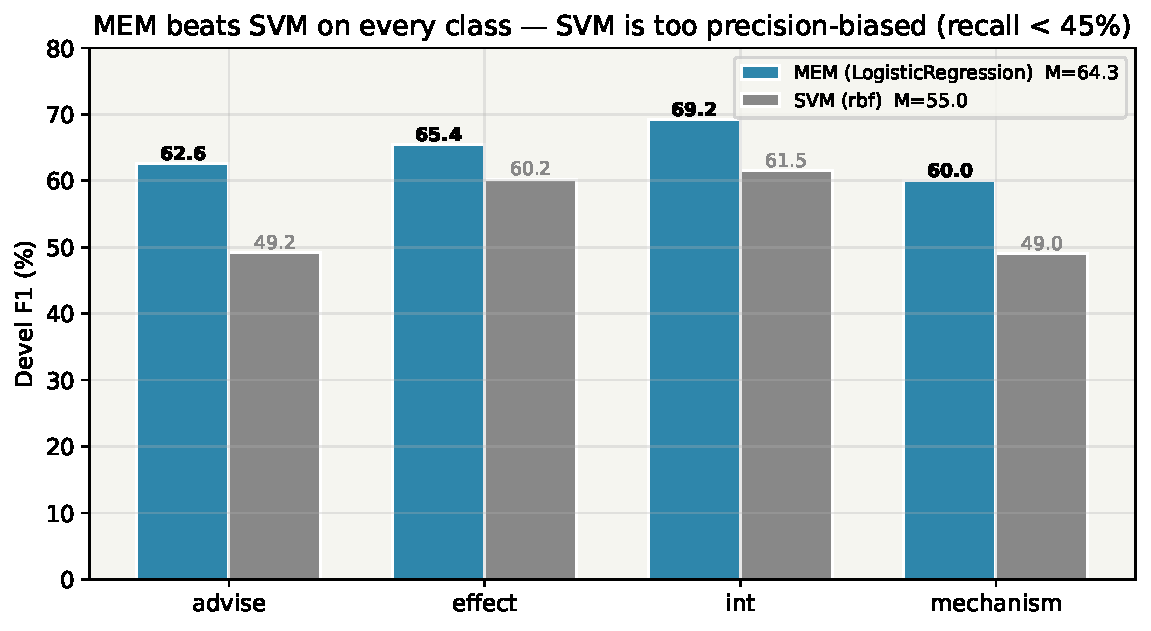
\includegraphics[width=0.78\linewidth]{fig21_mem_vs_svm.pdf}
\caption{MEM vs.\ SVM per-class F1 on devel. The high-dimensional, sparse feature space is exactly logistic regression's regime; the rbf-SVM under-fits the positive classes.}
\label{fig:memvssvm}
\end{figure}

\subsection{Feature-engineering experiments}
Following the brief's instruction to pay \emph{special attention to
syntax-based features}, we added feature mods one at a time on top of
the reference set and kept only those that helped on devel.

\begin{table}[H]
\centering\small
\renewcommand{\arraystretch}{1.18}
\rowcolors{2}{accentgrey!30}{white}
\begin{tabular}{>{\bfseries\color{upcblue}}l p{8.6cm} r}
\toprule
\rowcolor{upcblue}\textcolor{white}{\textbf{Mod}} & \textcolor{white}{\textbf{What it adds}} & \textcolor{white}{\textbf{$\Delta$M}} \\
\midrule
mod1 & distance + sentence-position / length buckets & $-$1.9 \\
mod2 & pharmacology clue-verbs (lemma + position vs.\ the pair) & $-$0.1 \\
mod3 & third-entity context (other entities in sentence / in path) & $-$0.3 \\
mod4 & combined entity-type pair feature (\texttt{typeE1\_typeE2}) & $-$0.2 \\
mod5 & negation cues near the LCS / in the path & $-$1.3 \\
\rowcolor{upclight}\textbf{mod\_best2} & \textbf{mod2 + mod3 together} & \textbf{+1.1} \\
\bottomrule
\end{tabular}
\caption{Additive feature mods, $\Delta$ macro-F1 vs.\ the reference (64.3). Every single mod is neutral-to-negative in isolation, but the \texttt{mod2+mod3} \emph{combination} (clue-verbs + third-entity context) synergises to +1.1\,pp. Adding \texttt{mod4} on top helps on test but hurts devel, so devel-selection keeps it out.}
\label{tab:featuremods}
\end{table}

\begin{figure}[H]
\centering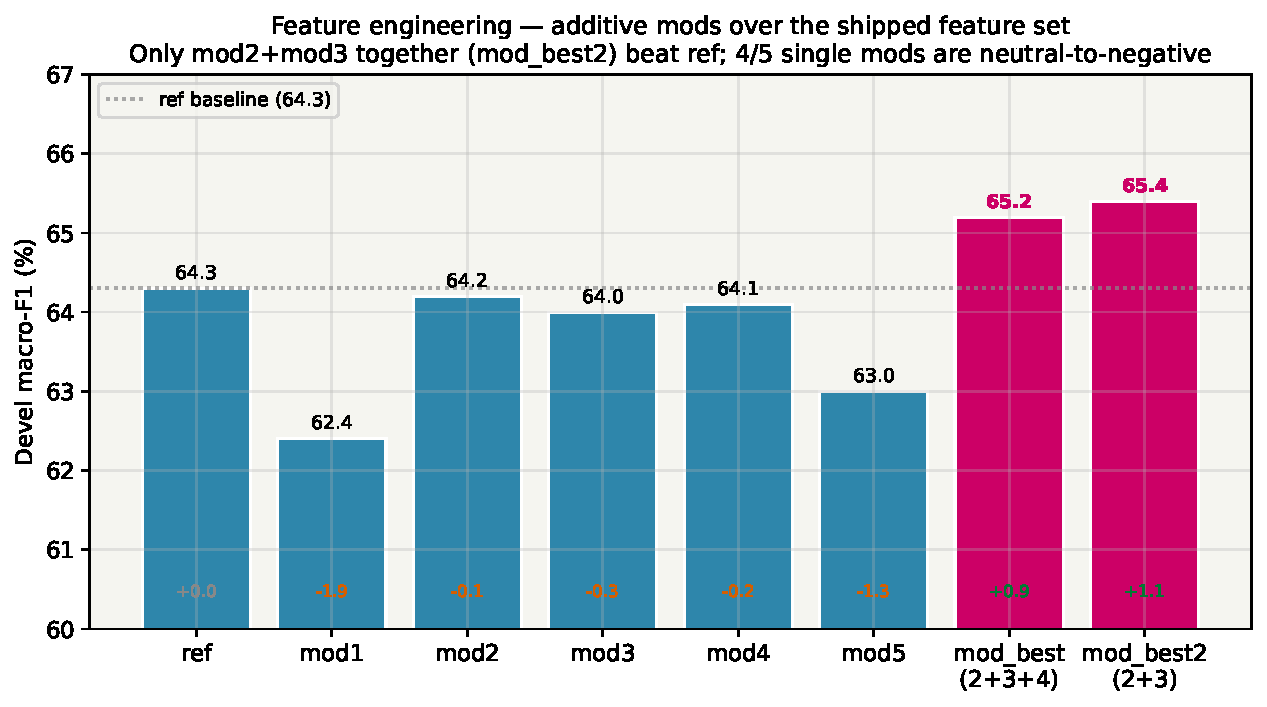
\includegraphics[width=0.92\linewidth]{fig21_feature_mods.pdf}
\caption{Feature-mod sweep on devel macro-F1. The lesson mirrors Task~1: the shipped feature set is already well-tuned, so isolated additions dilute a sparse model, but a carefully chosen \emph{combination} (\texttt{mod\_best2}) wins.}
\label{fig:featuremods}
\end{figure}

\begin{keybox}[Key observation]
The single most important finding of the feature campaign is that \textbf{combinations beat individuals}: \texttt{mod2} and \texttt{mod3} are each $\approx$neutral alone, yet together they lift macro-F1 by +1.1\,pp. The informative clue-verb and third-entity signals cooperate in a way the linear model cannot reconstruct from either one alone. A full hyperparameter sweep (solver $\in$ \{lbfgs, saga\}, $C\in[0.1,5]$, penalties l1/l2/elasticnet) added \emph{at most} +0.1\,pp on top --- \textbf{feature engineering, not hyperparameter tuning, is where the gains are}.
\end{keybox}

\subsection{The two-stage classifier - the largest single jump}
The reference is a flat 5-way classifier fighting both the
null-vs-positive imbalance \emph{and} the inter-positive boundary at
once. We decomposed it: \textbf{stage~1} is a binary
null-vs-positive router (logistic regression); \textbf{stage~2} is a
4-way classifier trained on positive-only data. A pair is routed to
stage~2 only when stage~1's $P(\text{positive})$ exceeds a threshold
tuned on devel.

\begin{figure}[H]
\centering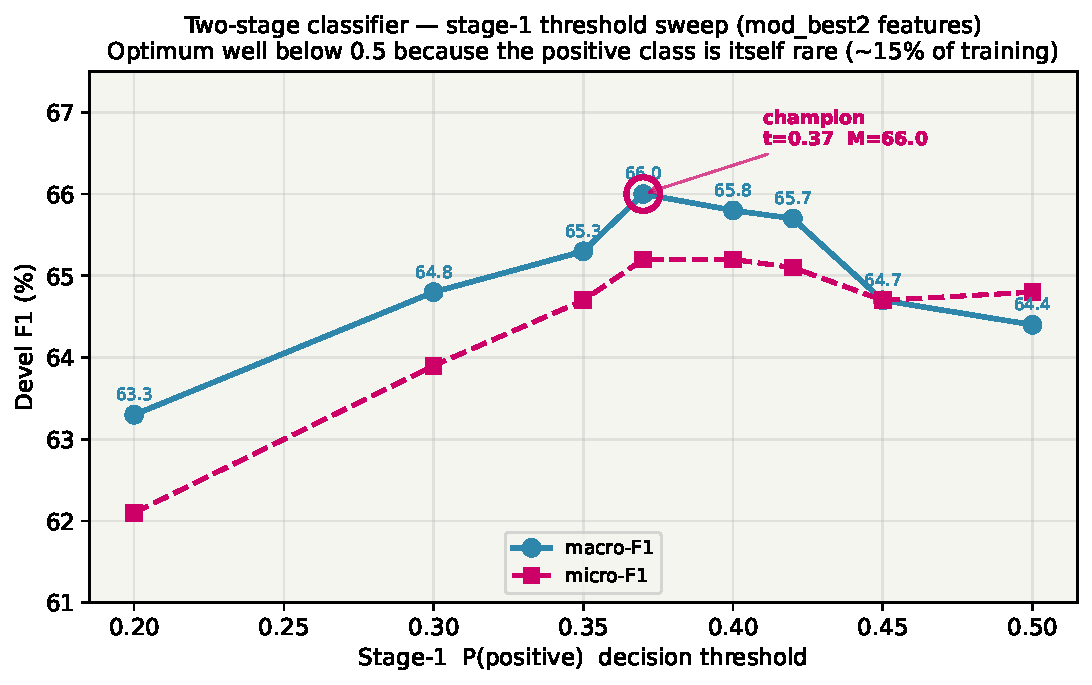
\includegraphics[width=0.74\linewidth]{fig21_threshold_sweep.pdf}
\caption{Stage-1 threshold sweep on devel. The optimum (\textbf{t = 0.37}, M-F1 = 66.0) sits well below 0.5 because the ``positive'' class is itself rare ($\approx$15\,\% of training pairs): demanding 0.5 probability would reject too many borderline true positives.}
\label{fig:threshold}
\end{figure}

The two-stage router at t = 0.37 is the \textbf{champion of System 2.1}:
devel M-F1 = 65.9, \textbf{test M-F1 = 66.8}, a +2.5\,pp devel and
+0.9\,pp test gain over the single-stage \texttt{mod\_best2}. It works
by trading precision for recall on every class --- exactly what we want
once stage~1, not the 4-way head, owns the imbalance decision.

\subsection{Best results, per-class and error analysis}

\begin{figure}[H]
\centering
\begin{subfigure}[t]{0.52\textwidth}
\centering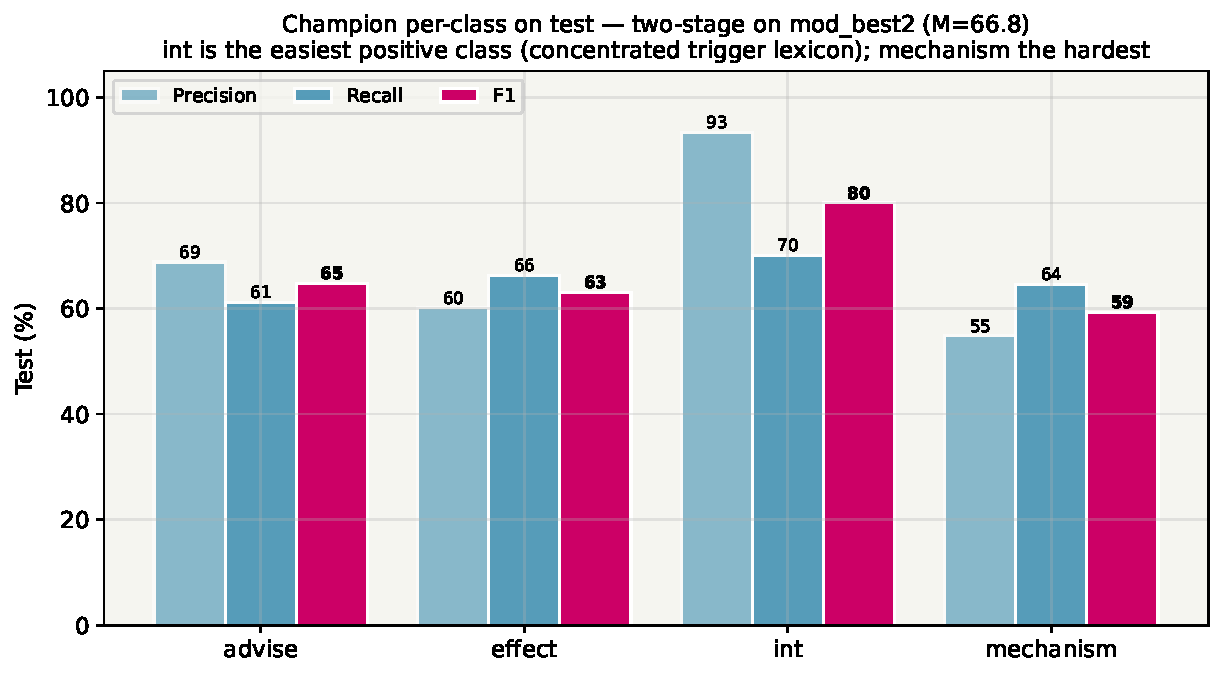
\includegraphics[width=\linewidth]{fig21_per_class_test.pdf}
\caption{Champion per-class P/R/F1 on test.}
\end{subfigure}\hfill
\begin{subfigure}[t]{0.46\textwidth}
\centering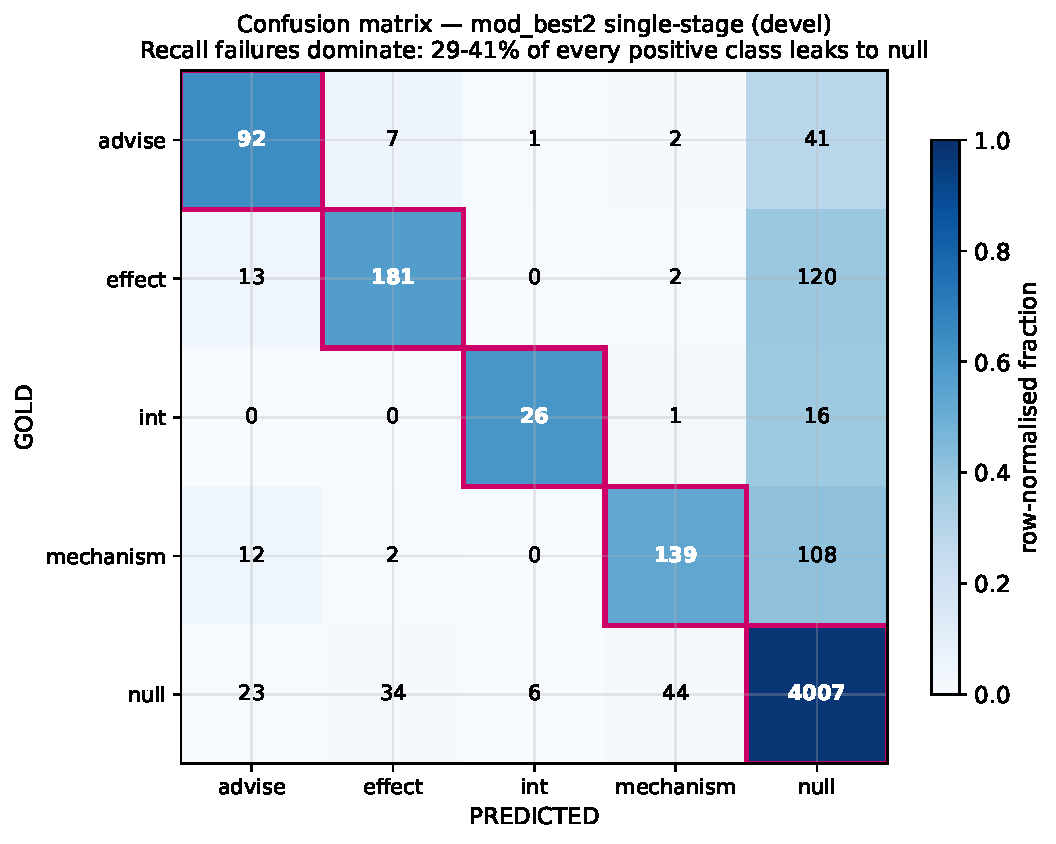
\includegraphics[width=\linewidth]{fig21_confmat.pdf}
\caption{Confusion matrix (\texttt{mod\_best2}, devel).}
\end{subfigure}
\caption{System 2.1 champion analysis. \texttt{int} is the easiest positive class (test F1 = 80.0, a concentrated trigger lexicon); \texttt{mechanism} is the hardest (diffuse phrasing). The confusion matrix shows the dominant error is \emph{recall} failure --- 29--41\,\% of every positive class leaks to \texttt{null} --- not inter-positive confusion, which is small.}
\label{fig:ml-champ}
\end{figure}

\begin{figure}[H]
\centering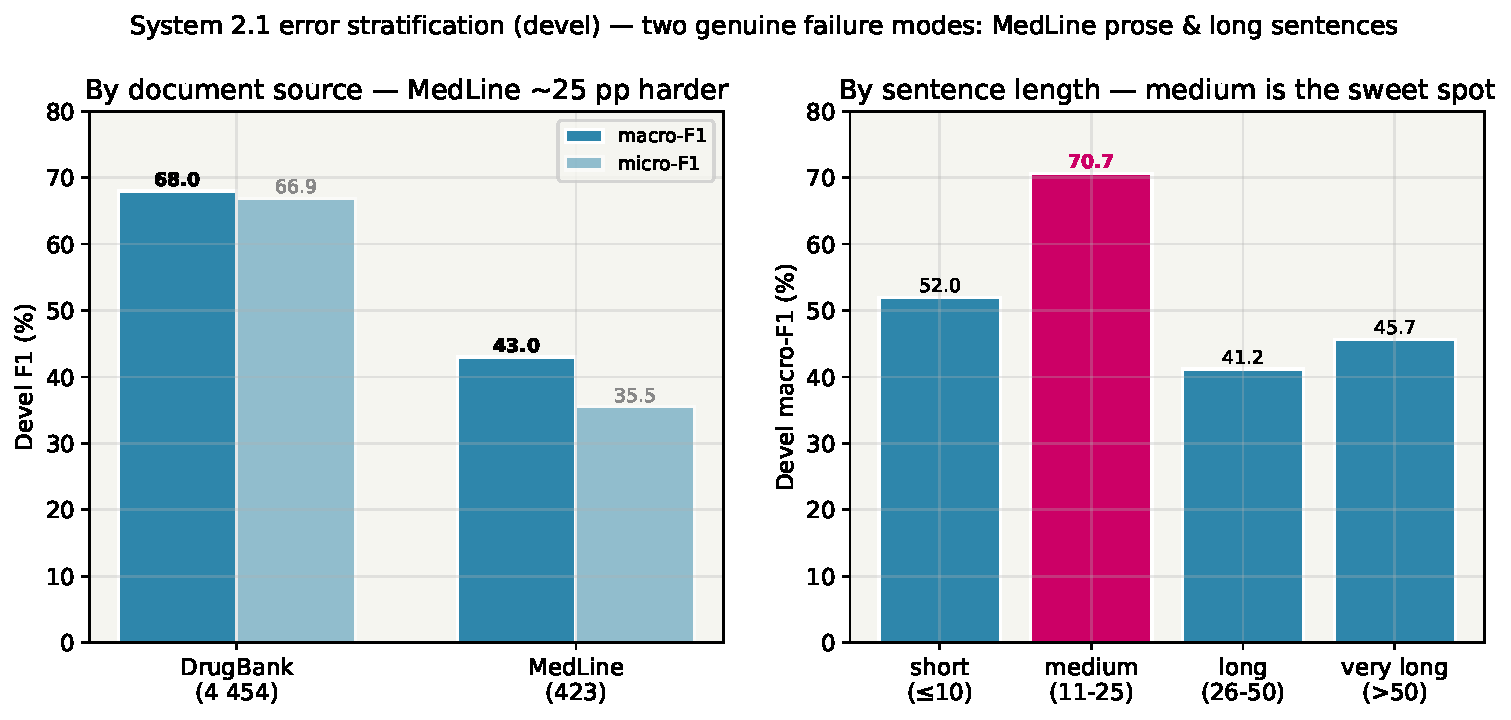
\includegraphics[width=\linewidth]{fig21_strata.pdf}
\caption{Error stratification on devel. \textbf{DrugBank pairs are $\approx$25\,pp easier than MedLine} (standardised drug-label phrasing fits the clue-verb features; research-abstract prose does not), and \textbf{medium-length sentences are the sweet spot} --- both very short (too few words for the verb features to fire) and long ($>$25 words, noisy dependency paths) sentences are harder.}
\label{fig:ml-strata}
\end{figure}

\begin{keybox}[Deep dive --- five extensions that all fall short]
After the headline, we tried five further refinements: stage-2
class-balancing, train+devel re-training, per-class thresholds, a
mechanism-specific trigger lexicon (\texttt{mod8}), and single/two-stage
ensembling. \emph{Per-class thresholds} gave a spectacular +2.5\,pp on
\textbf{devel} but $-$1.5\,pp on \textbf{test} --- the four free
thresholds overfit the $\sim$700 devel positives. Every extension
showed the same pattern: devel gains that do not survive test. At this
data scale, the single global threshold acts as an implicit regulariser,
and the plain two-stage classifier is the honest, devel-selected
champion.
\end{keybox}

\subsection{Discussion}
Inspecting the learned weights confirms the classifier is well-behaved:
the strongest single feature in the whole model is \texttt{same-drug}
(a drug mentioned twice is almost never a real interaction), and each
class's top features are linguistically sensible (modal verbs
``\textit{should}'' for \texttt{advise}; pharmacokinetic vocabulary
``\textit{absorption}'', ``\textit{metabolism}'' for \texttt{mechanism}).
The two genuine failure modes are MedLine-style research prose and long
sentences with diffuse syntax --- both out-of-domain for the shipped
syntactic feature set. \textbf{System 2.1 final: two-stage on
\texttt{mod\_best2}, lbfgs, t = 0.37 $\to$ test M-F1 = 66.8} (+39.9\,pp
over the rule-based 2.0).

%% ============================================================
\section{System 2.2 - DDI with Neural Networks}\label{sec:nn}
%% ============================================================

\subsection{Starting point}
The shipped network (despite being called ``CNN'' in the brief) is a
\textbf{BiLSTM-then-CNN hybrid}: three embedded input channels
(lower-cased word, lemma, PoS) are concatenated, run through a
BiLSTM(250$\to$200), then a 1-D convolution and a global max-pool, and a
linear layer projects to the 5 classes. Crucially, the network sees
\emph{only} word/lemma/PoS sequences --- it has \textbf{none} of the
dependency-path features that carry most of the DDI signal in 2.1. The
reference network reaches devel M-F1 = 55.8, fully \textbf{10\,pp below
the ML reference}, and this gap defines the opportunity.

\subsection{Input-representation experiments}
The brief asks us to experiment with input encodings; this turned out to
be by far the largest lever.

\begin{figure}[H]
\centering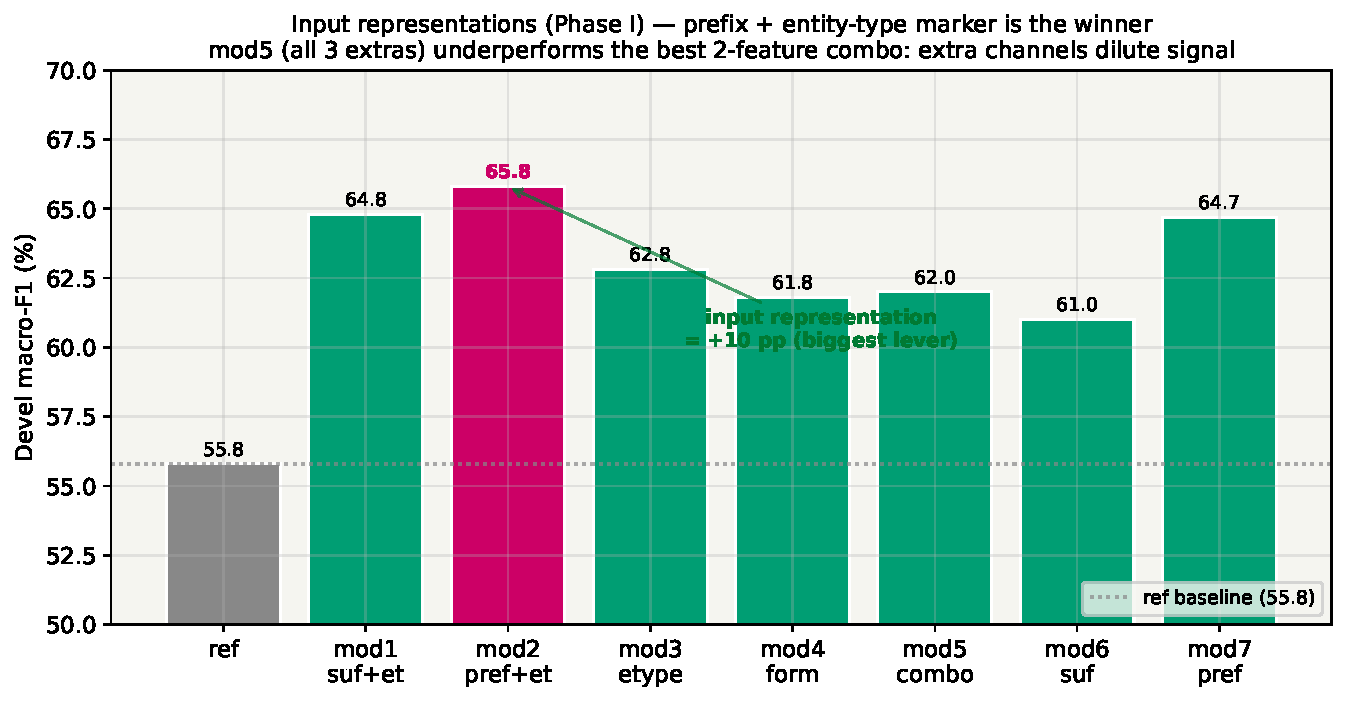
\includegraphics[width=0.95\linewidth]{fig22_input_mods.pdf}
\caption{Phase~I input-representation sweep (devel macro-F1). Adding a \textbf{prefix-3 channel plus an entity-type marker} (\texttt{mod2}) lifts macro-F1 by \textbf{+10\,pp} over the shipped baseline --- the single biggest improvement anywhere in System 2.2. Combining all three extra channels (\texttt{mod5}) does \emph{worse} than the best two-channel combo: at this data scale extra input channels dilute the signal.}
\label{fig:nn-inputs}
\end{figure}

\subsection{Architecture and hyperparameter experiments}

\begin{figure}[H]
\centering
\begin{subfigure}[t]{0.52\textwidth}
\centering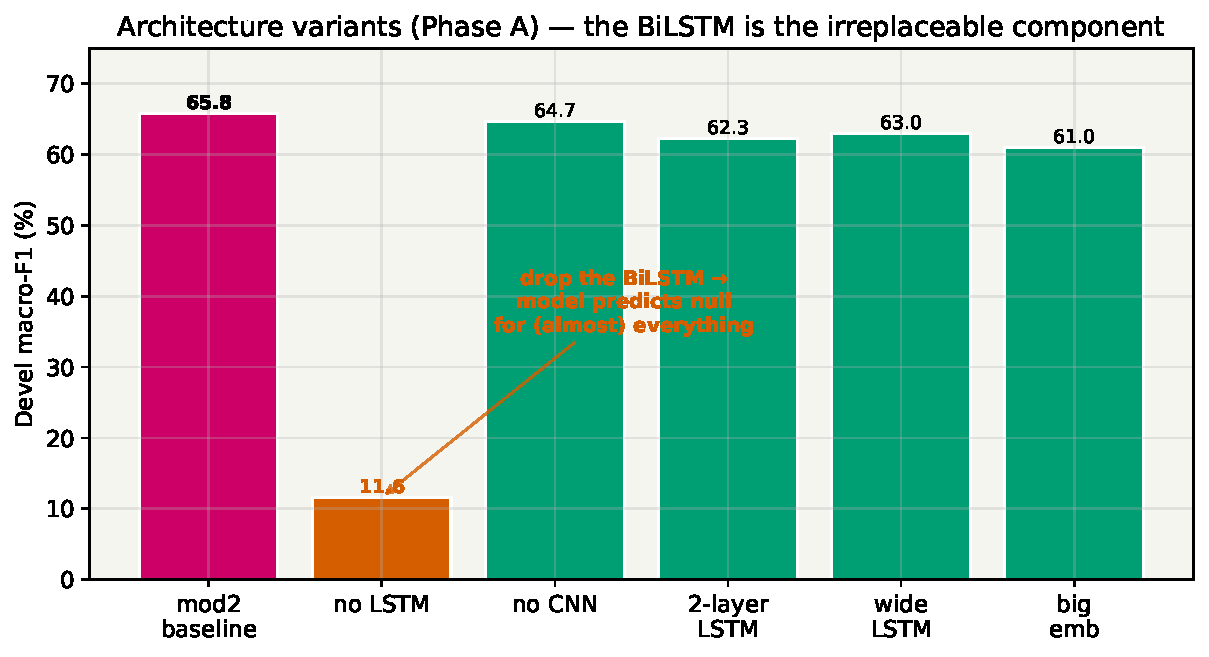
\includegraphics[width=\linewidth]{fig22_arch.pdf}
\caption{Architecture variants.}
\end{subfigure}\hfill
\begin{subfigure}[t]{0.46\textwidth}
\centering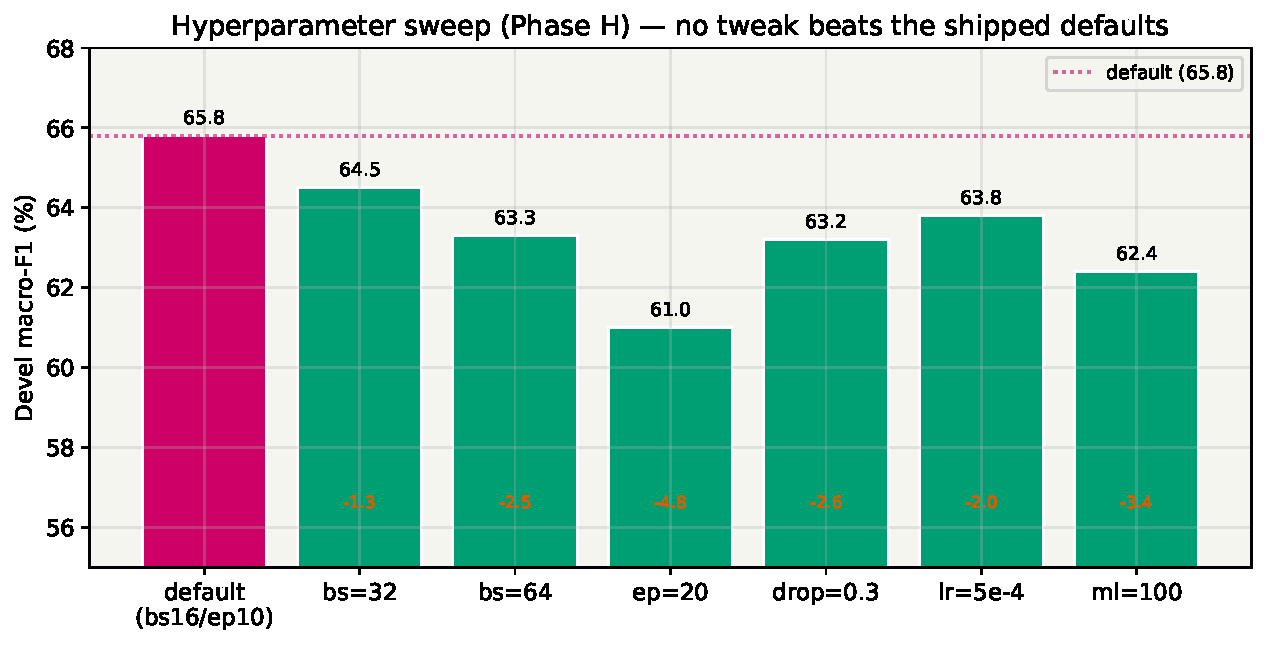
\includegraphics[width=\linewidth]{fig22_hp.pdf}
\caption{Hyperparameter sweep.}
\end{subfigure}
\caption{Phase~A/H. \textbf{Removing the BiLSTM collapses the model to M-F1 = 11.6} (it predicts \texttt{null} for almost everything) --- the BiLSTM is the irreplaceable component, while the CNN contributes only $\approx$1\,pp. No depth/width change and no hyperparameter tweak beats the shipped defaults; deeper/wider variants overfit at this data scale.}
\label{fig:nn-arch}
\end{figure}

\subsection{Relative-position embedding - the champion modification}
The deep dive's most impactful idea was a \textbf{relative-position
embedding} (\texttt{mod9}): for every token, embed its bucketed distance
to \texttt{<DRUG1>} and to \texttt{<DRUG2>}. This gives the network the
explicit ``near the pair vs.\ far away'' signal that a plain BiLSTM
lacks --- a standard relation-extraction trick.

\begin{figure}[H]
\centering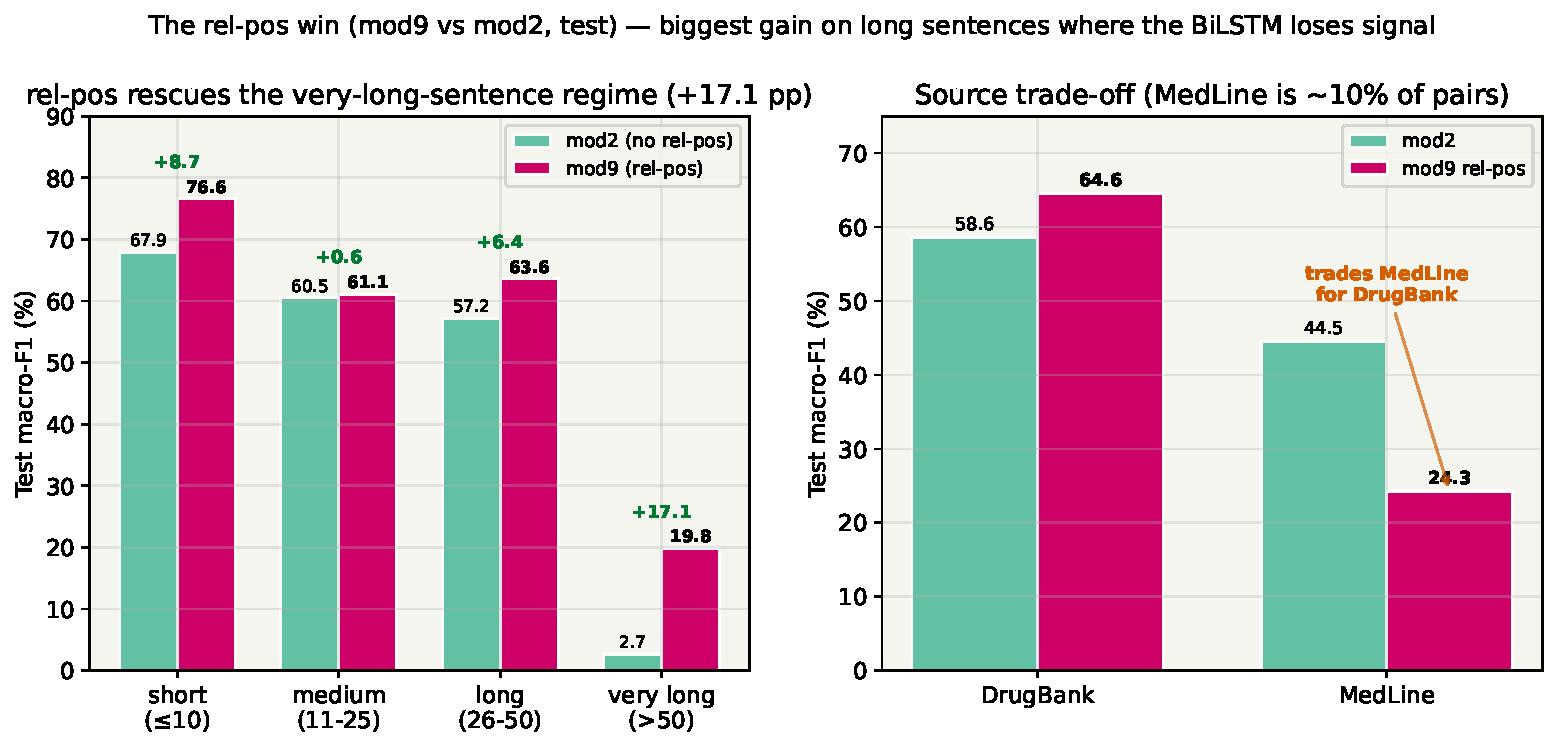
\includegraphics[width=\linewidth]{fig22_relpos_strata.pdf}
\caption{Relative-position (\texttt{mod9}) vs.\ \texttt{mod2} on test. Rel-pos rescues exactly the regime the BiLSTM struggles with: \textbf{+17.1\,pp on very-long sentences} (from a near-dead 2.7 to 19.8) and +6.4\,pp on long ones. It trades away some MedLine accuracy (a small $\approx$10\,\% subset) for a large DrugBank and long-sentence gain.}
\label{fig:nn-relpos}
\end{figure}

\subsection{The seed lottery - a critical methodological finding}
A multi-seed audit revealed that single-seed devel selection is
unreliable on this small dataset.

\begin{figure}[H]
\centering
\begin{subfigure}[t]{0.62\textwidth}
\centering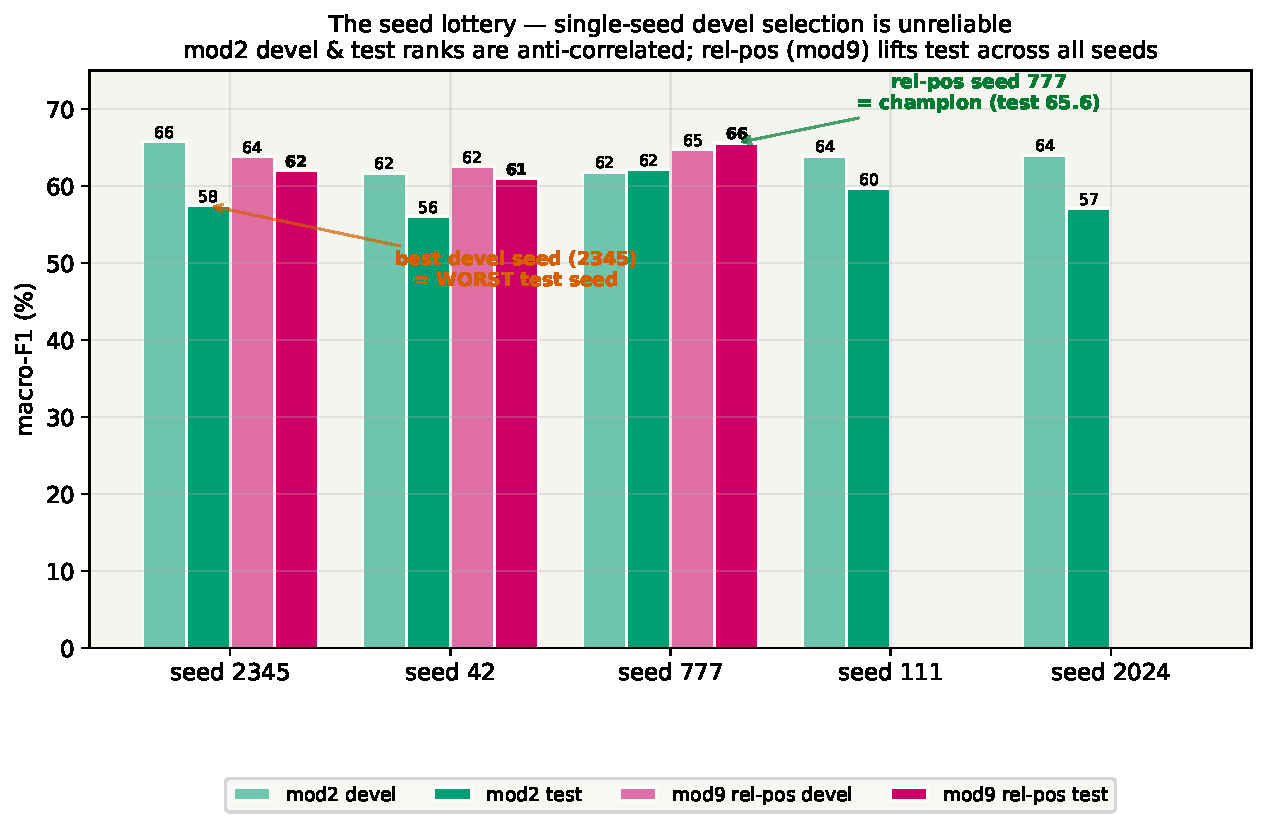
\includegraphics[width=\linewidth]{fig22_seed_audit.pdf}
\caption{Seed audit: devel vs.\ test across seeds.}
\end{subfigure}\hfill
\begin{subfigure}[t]{0.36\textwidth}
\centering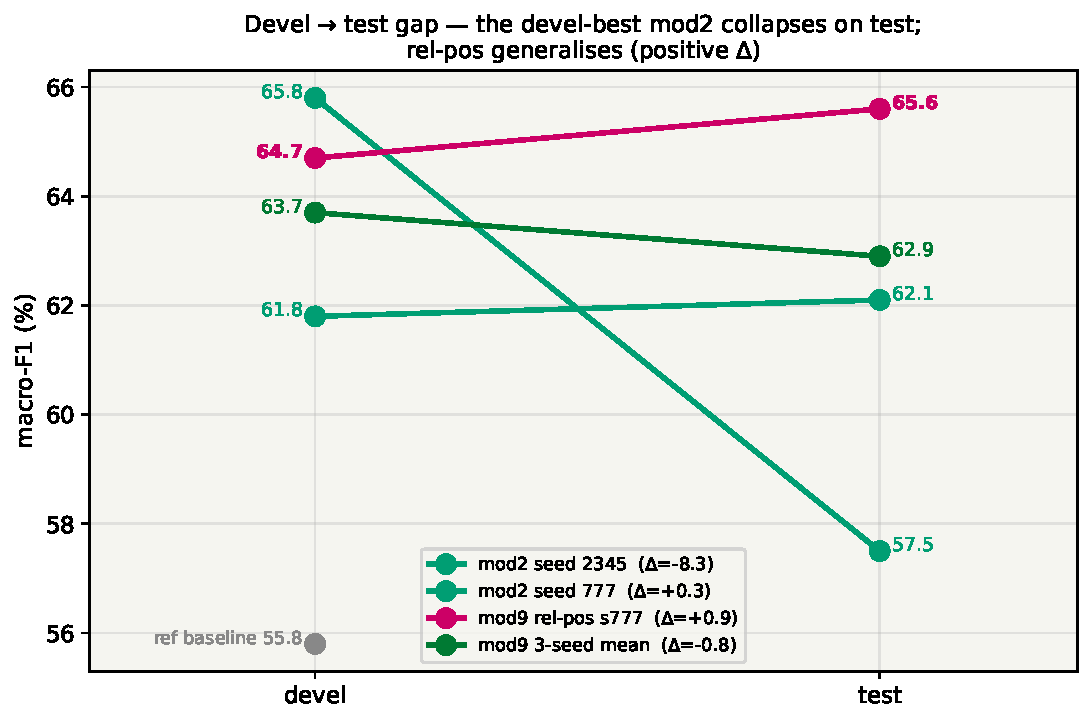
\includegraphics[width=\linewidth]{fig22_devel_test_gap.pdf}
\caption{Devel$\to$test slope, key configs.}
\end{subfigure}
\caption{The \texttt{mod2} devel-best seed (2345) is a +2.4$\sigma$ outlier on devel and the \emph{worst} seed on test --- devel and test ranks are anti-correlated. The relative-position model (\texttt{mod9}), by contrast, generalises positively across all seeds. Its devel-selected seed (777) is the System 2.2 champion.}
\label{fig:nn-seed}
\end{figure}

\subsection{Best results and discussion}

\begin{figure}[H]
\centering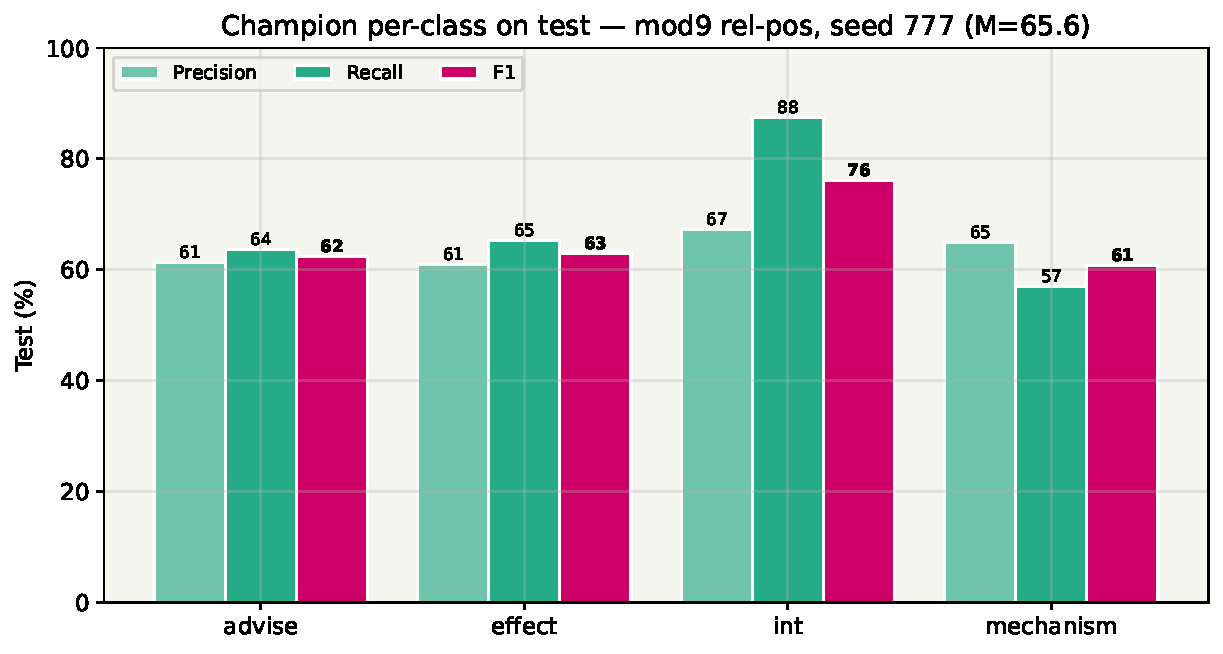
\includegraphics[width=0.62\linewidth]{fig22_per_class_test.pdf}
\caption{System 2.2 champion (\texttt{mod9} rel-pos, seed 777) per-class on test, M-F1 = 65.6. As in 2.1, \texttt{int} is the strongest class (F1 = 76.1).}
\label{fig:nn-champ}
\end{figure}

\begin{okbox}
\textbf{System 2.2 final: BiLSTM + relative-position embedding, devel-selected seed 777 $\to$ test M-F1 = 65.6}, within 1.2\,pp of the ML champion. The relative-position embedding is the single most impactful change (biggest test gain in the campaign), and a clean architectural conclusion emerges: \textbf{relative position and the BiLSTM are complementary, not interchangeable} --- a pure CNN with rel-pos but no BiLSTM collapses to 0.0. The recurring lesson is the same as 2.1: \emph{input representation $>$ architecture $>$ hyperparameters}, and single-seed peaks must be treated with suspicion.
\end{okbox}

%% ============================================================
\section{System 2.3 - DDI with Large Language Models}\label{sec:llm}
%% ============================================================

\subsection{Starting point and output format}
The LLM system frames DDI as \textbf{single-label generation}: the two
target drugs are masked in the sentence as \texttt{[DRUG1]} /
\texttt{[DRUG2]} (other entities as \texttt{[DRUG\_OTHER]}), and the
model is asked to emit exactly one of the five class labels. We work
with two 4-bit-quantised 3B instruction models, \textbf{Llama-3.2-3B}
and \textbf{Qwen-2.5-3B}, on the Boada cluster. The brief asks us to
experiment along three axes: prompt adaptation, few-shot example
selection, and fine-tuning (examples + hyperparameters).

\subsection{Few-shot experiments}

\begin{figure}[H]
\centering
\begin{subfigure}[t]{0.52\textwidth}
\centering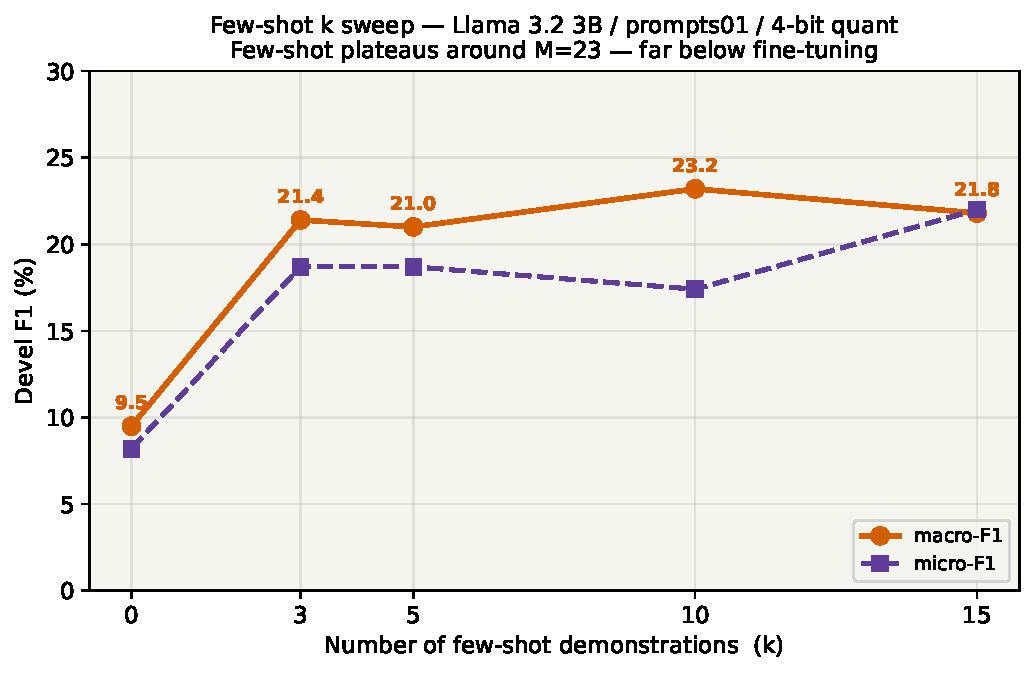
\includegraphics[width=\linewidth]{fig23_fs_sweep.pdf}
\caption{Few-shot $k$-sweep (Llama, \texttt{prompts01}).}
\end{subfigure}\hfill
\begin{subfigure}[t]{0.46\textwidth}
\centering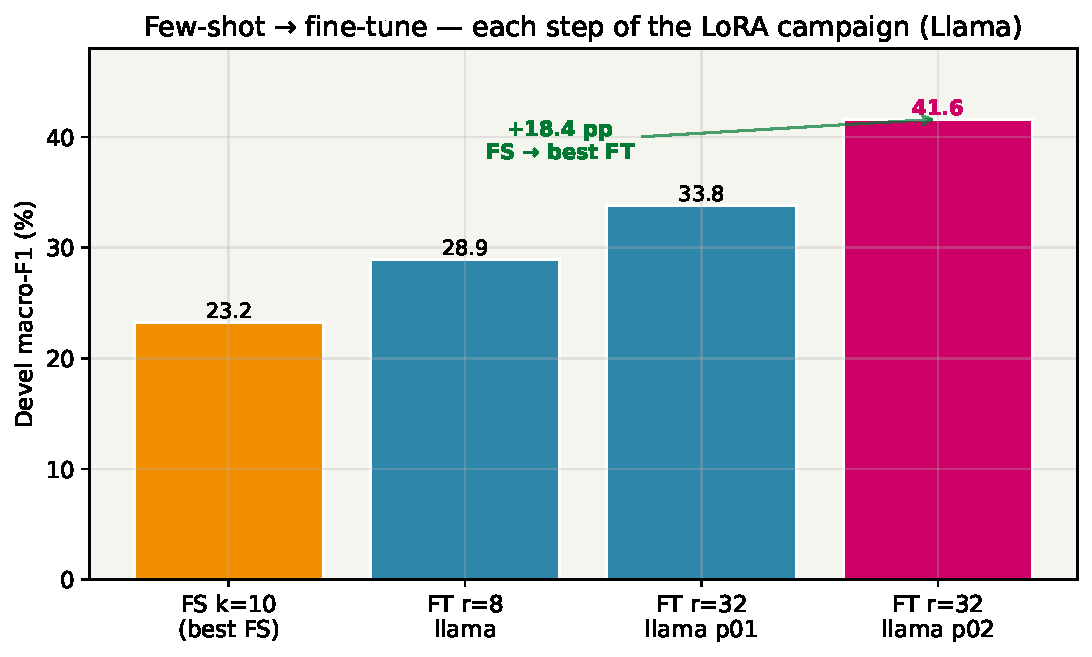
\includegraphics[width=\linewidth]{fig23_fs_vs_ft.pdf}
\caption{Few-shot $\to$ fine-tune jump.}
\end{subfigure}
\caption{Few-shot inference plateaus around macro-F1 = 23 regardless of the number of demonstrations $k$ --- far below even the weakest fine-tune. Fine-tuning is essential: each step of the LoRA campaign adds clear macro-F1.}
\label{fig:llm-fs}
\end{figure}

\subsection{Fine-tuning experiments}
We fine-tuned both models with LoRA at two ranks ($r{=}8$, $r{=}32$,
$\alpha{=}2r$) and two prompt templates. \texttt{prompts02} fixes a typo
in the \texttt{advise} class definition and strengthens the
``do not invent an interaction'' instruction for \texttt{null}.

\begin{figure}[H]
\centering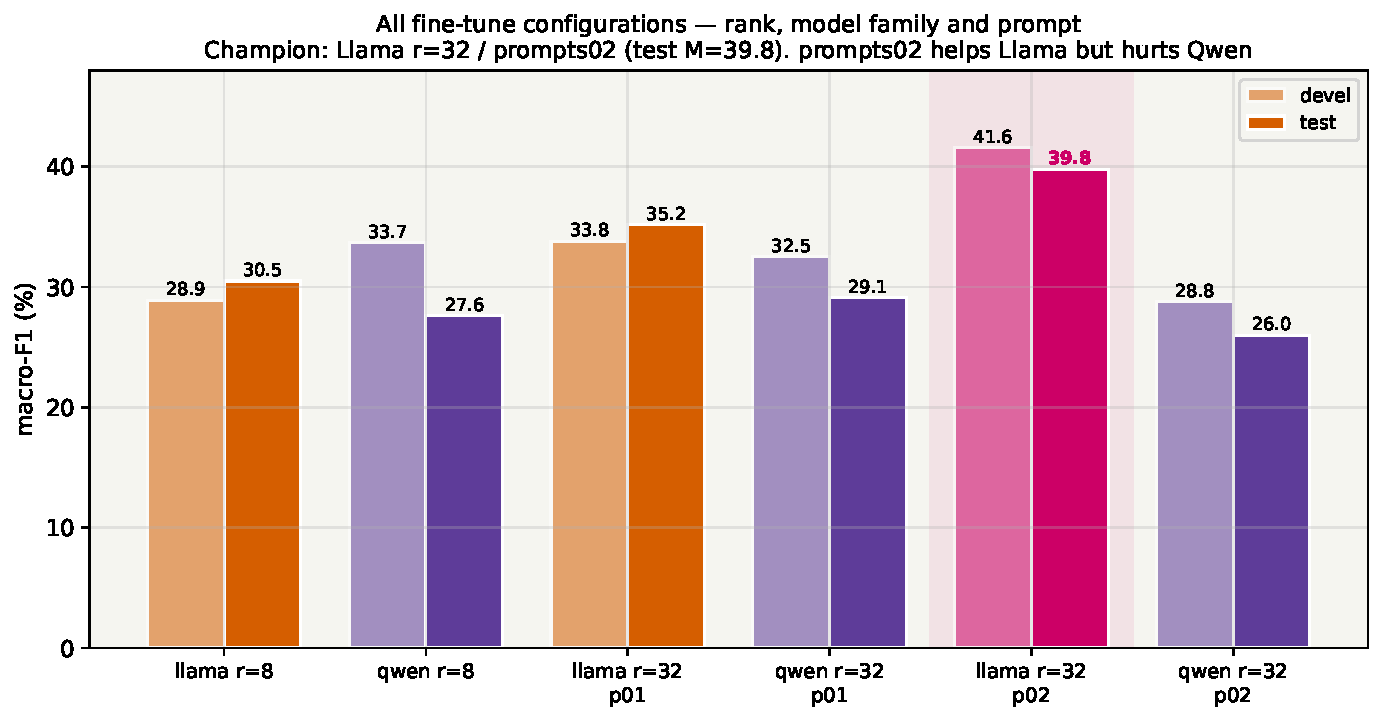
\includegraphics[width=0.95\linewidth]{fig23_ft_configs.pdf}
\caption{All fine-tune configurations (devel + test macro-F1). The champion is \textbf{Llama $r{=}32$ / \texttt{prompts02} (test M-F1 = 39.8)}. Doubling the LoRA rank ($8\to32$) and improving the prompt each add $\approx$+5\,pp on Llama --- prompt quality is as powerful a lever as adapter capacity.}
\label{fig:llm-ft}
\end{figure}

\subsection{Prompt brittleness across model families - a key finding}
The most interesting result of the campaign is that the \emph{same}
prompt improvement has \emph{opposite} effects on the two model families.

\begin{figure}[H]
\centering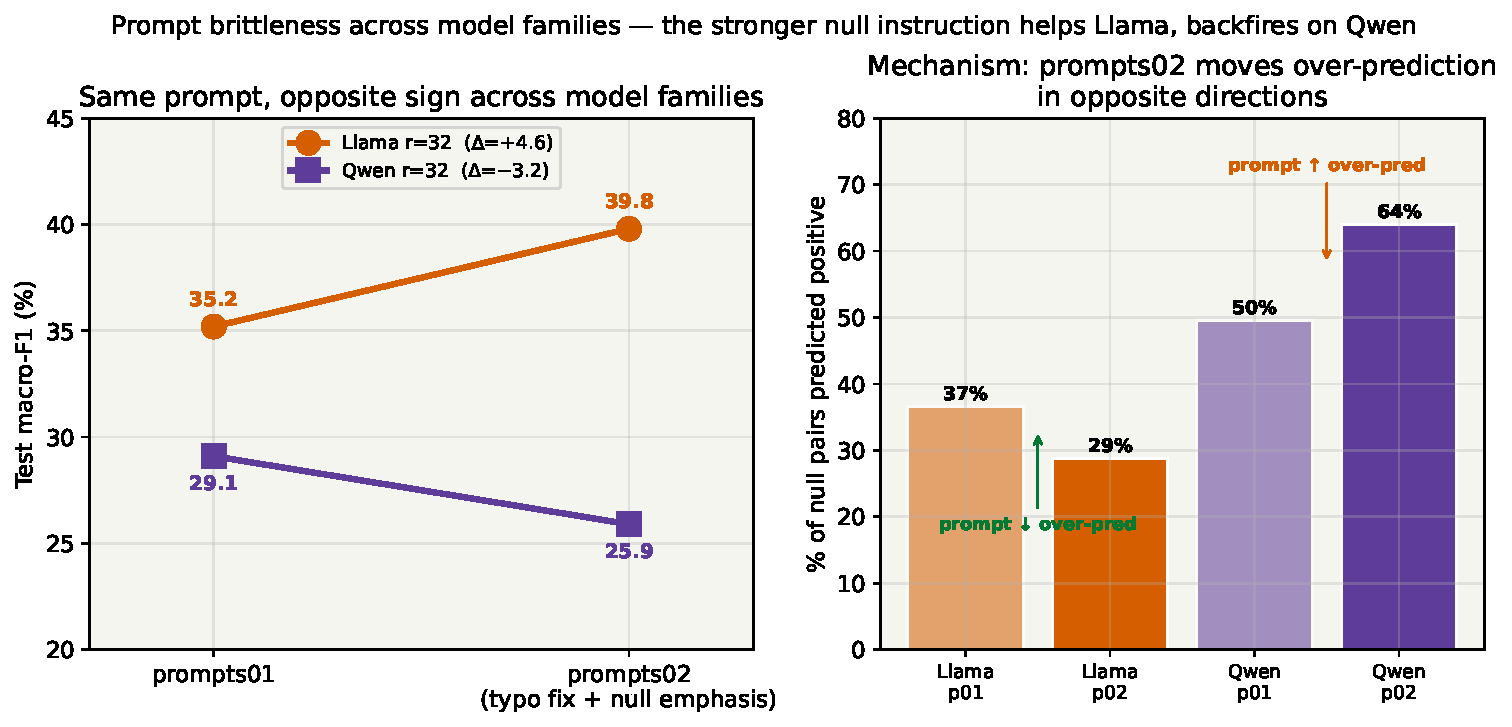
\includegraphics[width=\linewidth]{fig23_prompt_crossmodel.pdf}
\caption{\texttt{prompts02} helps Llama (+4.6\,pp test) but \emph{hurts} Qwen ($-$3.2\,pp). The mechanism (right) is the null over-prediction rate: the stronger \texttt{null} instruction made Llama predict positives \emph{less} (36.6\,\%$\to$28.8\,\%) but made Qwen predict them \emph{more} (49.6\,\%$\to$64\,\%). The same instruction is read as caution by one model and as licence by the other.}
\label{fig:llm-prompt}
\end{figure}

\begin{figure}[H]
\centering
\begin{subfigure}[t]{0.48\textwidth}
\centering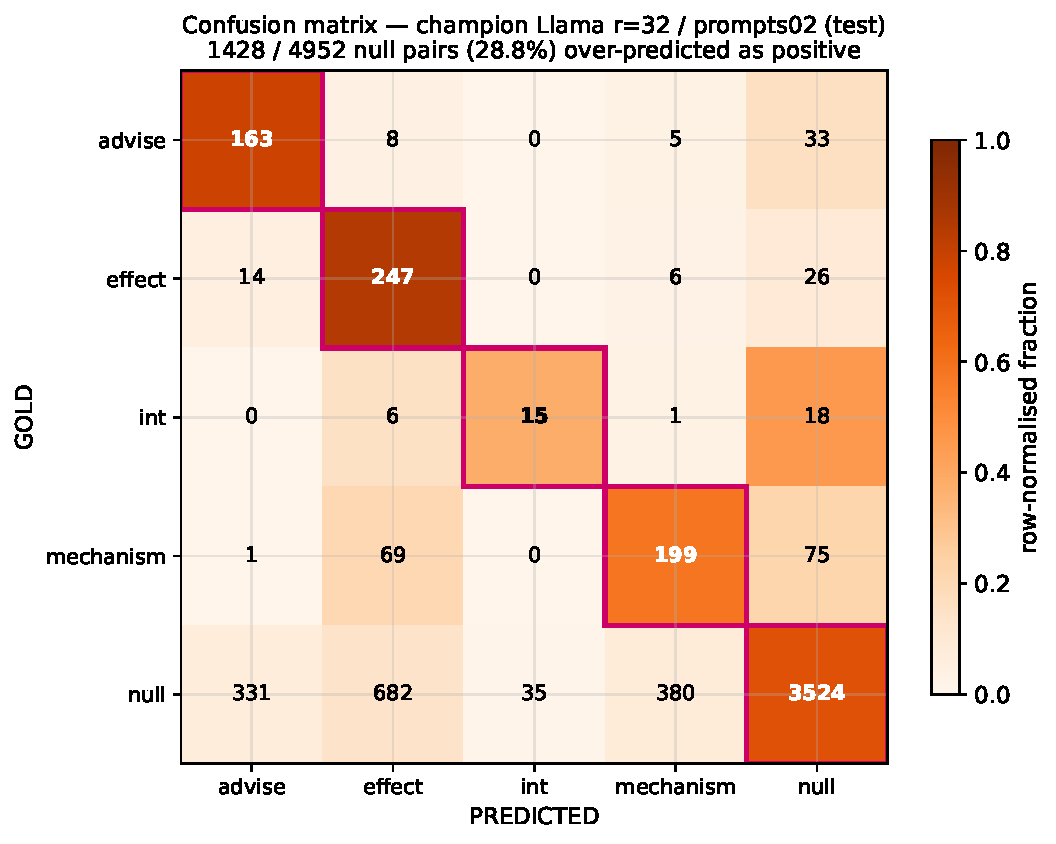
\includegraphics[width=\linewidth]{fig23_confmat.pdf}
\caption{Champion confusion matrix (test).}
\end{subfigure}\hfill
\begin{subfigure}[t]{0.50\textwidth}
\centering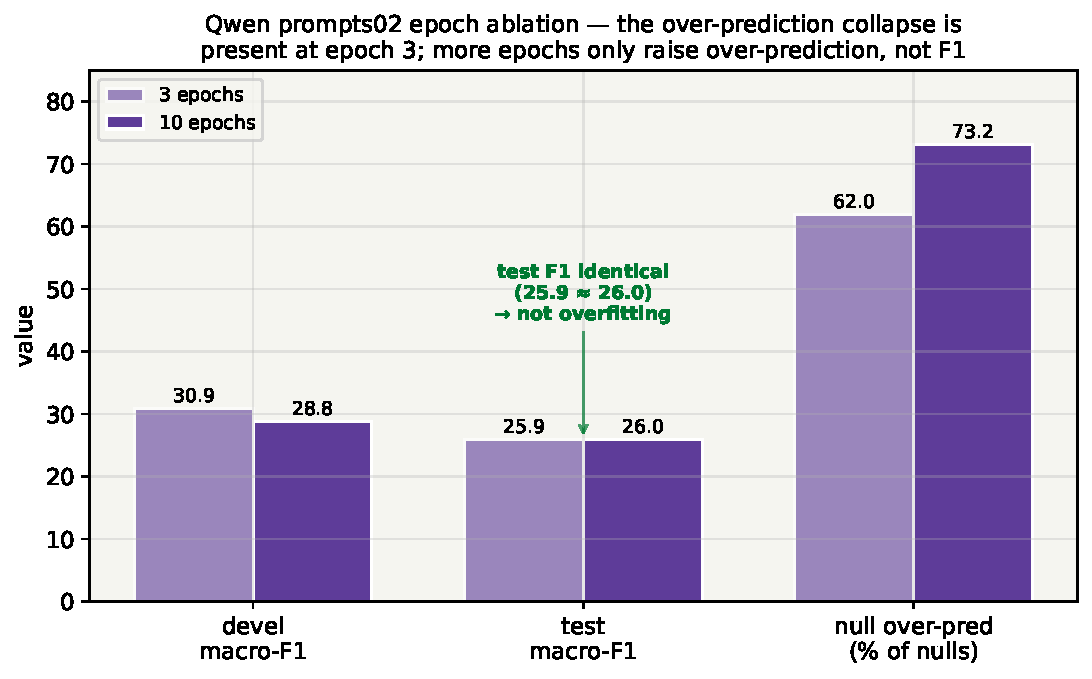
\includegraphics[width=\linewidth]{fig23_epoch_ablation.pdf}
\caption{Qwen epoch ablation.}
\end{subfigure}
\caption{Left: even the champion over-predicts --- 28.8\,\% of all \texttt{null} pairs receive a positive label (precision $\ll$ recall on every class). Right: a 3-epoch vs.\ 10-epoch ablation on Qwen shows the over-prediction collapse is \emph{not} overfitting --- test F1 is identical (25.9 vs.\ 26.0); more epochs only inflate the over-prediction rate.}
\label{fig:llm-confmat}
\end{figure}

\subsection{A negative result and error stratification}

\begin{figure}[H]
\centering
\begin{subfigure}[t]{0.50\textwidth}
\centering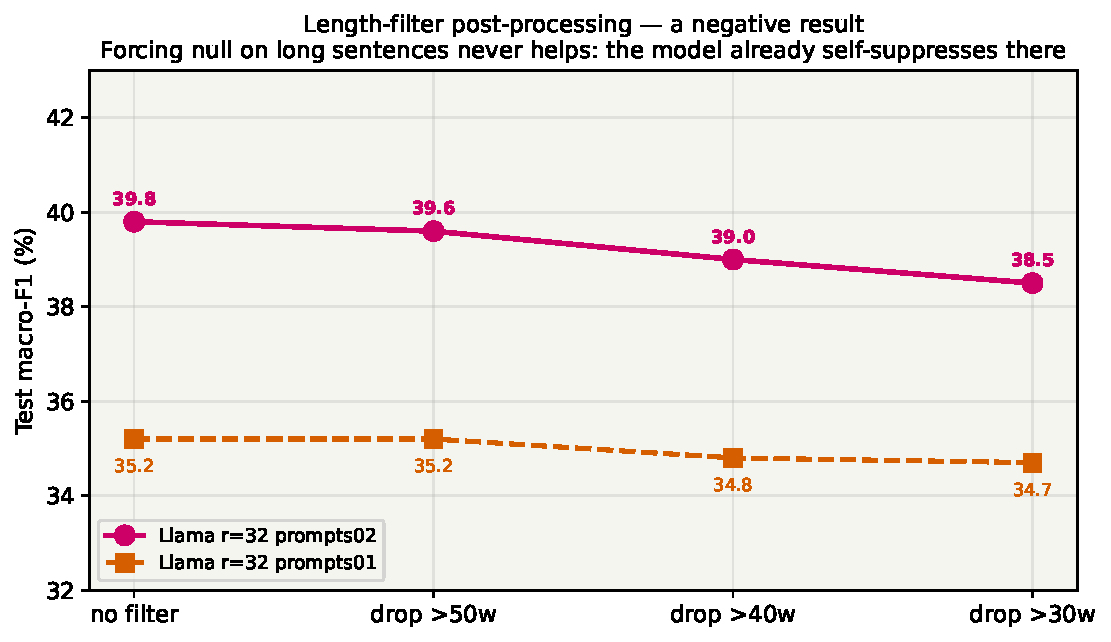
\includegraphics[width=\linewidth]{fig23_length_filter.pdf}
\caption{Length-filter post-processing (negative).}
\end{subfigure}\hfill
\begin{subfigure}[t]{0.48\textwidth}
\centering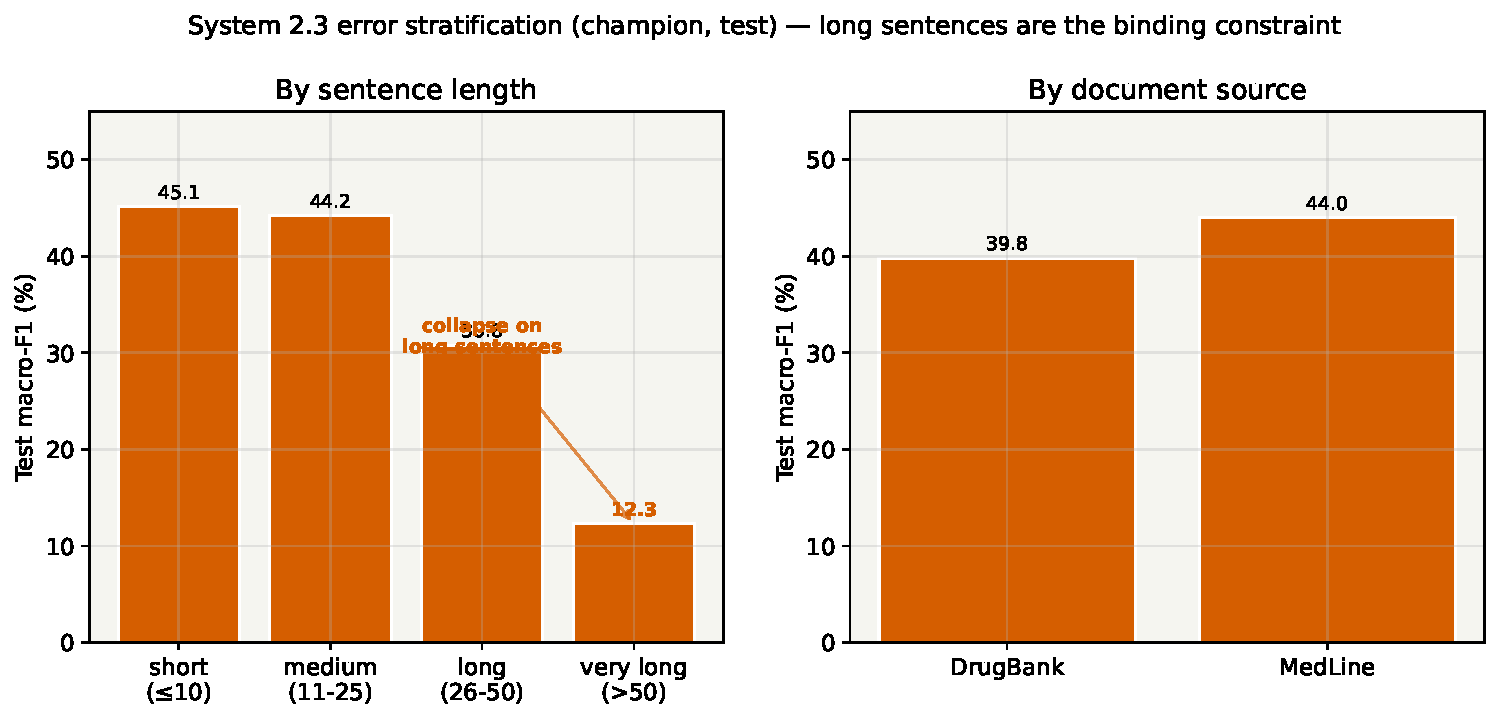
\includegraphics[width=\linewidth]{fig23_strata.pdf}
\caption{Error stratification (champion, test).}
\end{subfigure}
\caption{Left: forcing \texttt{null} on long sentences never helps --- the model already self-suppresses there (only $\approx$2\,\% of its positive predictions fall in $>$50-word sentences), so the collapse is a \emph{recall} problem, not a precision one a filter could fix. Right: like 2.1 and 2.2, the LLM degrades sharply on long sentences (M-F1 = 12.3 on $>$50 words).}
\label{fig:llm-neg}
\end{figure}

\begin{okbox}
\textbf{System 2.3 final: LoRA fine-tuned Llama-3.2-3B, $r{=}32$, \texttt{prompts02} $\to$ test M-F1 = 39.8.} Three transferable findings: (1) fine-tuning is mandatory --- few-shot plateaus 17\,pp lower; (2) prompt quality is a first-class capacity lever, as strong as LoRA rank, but it is \textbf{not transferable across model families} (it helped Llama and hurt Qwen); (3) the binding constraint is the positive/\texttt{null} boundary --- the model over-predicts interactions, and no inference-time guardrail repairs it.
\end{okbox}

%% ============================================================
\section{Conclusions: Cross-System Comparison}\label{sec:conclusions}
%% ============================================================

All three systems attack the \emph{same} DDI task and are scored by the
\emph{same} evaluator on the \emph{same} test split, so the numbers are
directly comparable.

\subsection{Headline test-set results}

\begin{figure}[H]
\centering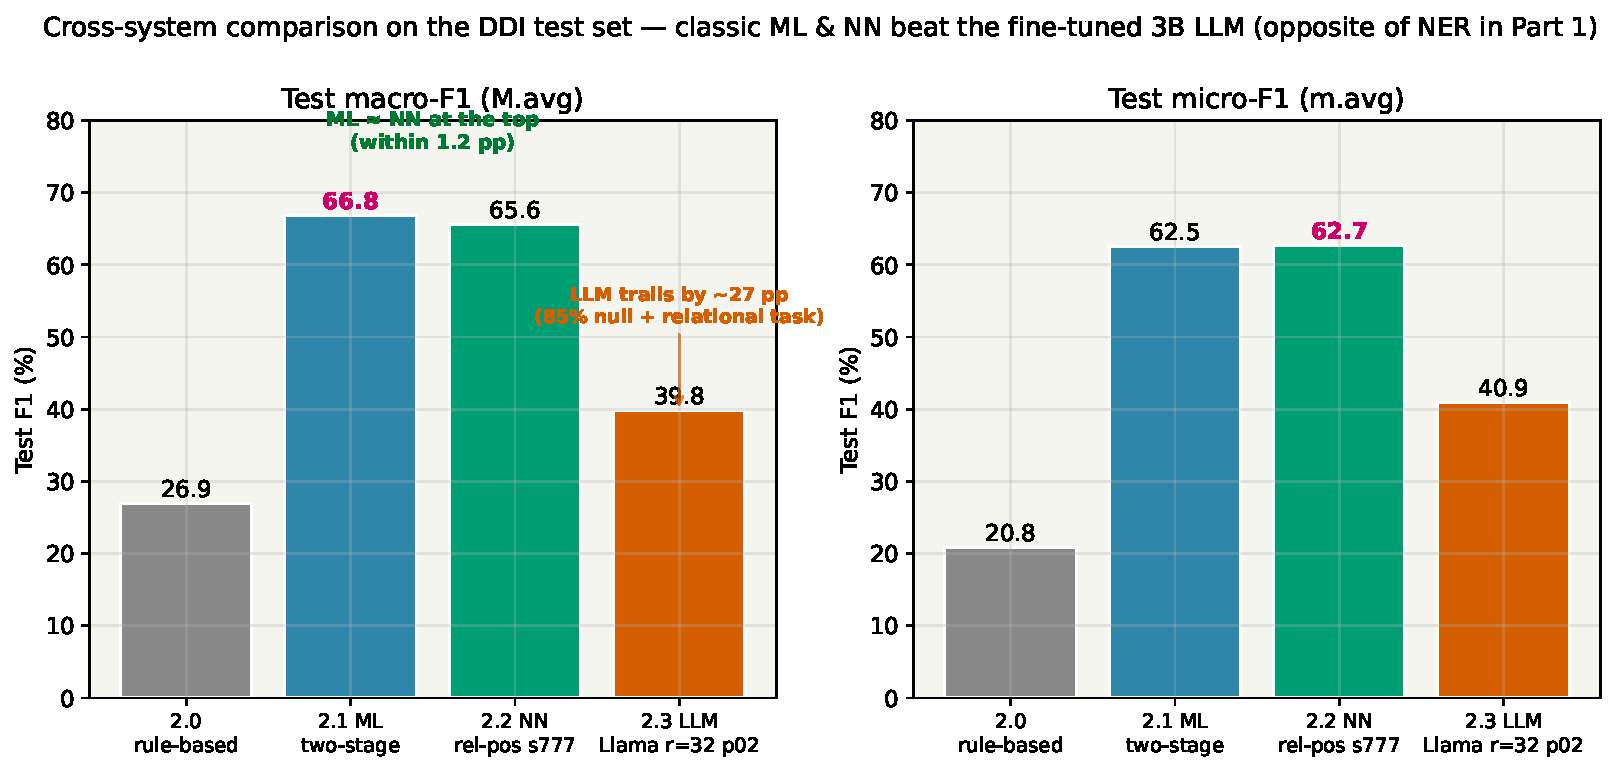
\includegraphics[width=\linewidth]{fig2_cross_system.pdf}
\caption{Cross-system test F1. The classical ML system wins macro-F1 (66.8), the neural network is within 1.2\,pp (65.6), and the fine-tuned 3B LLM trails both by $\approx$27\,pp (39.8). This is the \emph{mirror image} of Task~1 (NERC), where the fine-tuned LLM won macro-F1 outright.}
\label{fig:cross}
\end{figure}

\begin{table}[H]
\centering\small
\renewcommand{\arraystretch}{1.2}
\rowcolors{2}{accentgrey!30}{white}
\begin{tabular}{>{\bfseries\color{upcblue}}l r r r r r r}
\toprule
\rowcolor{upcblue}\textcolor{white}{\textbf{System (test)}} & \textcolor{white}{\textbf{M-F1}} & \textcolor{white}{\textbf{m-F1}} & \textcolor{white}{\textbf{advise}} & \textcolor{white}{\textbf{effect}} & \textcolor{white}{\textbf{int}} & \textcolor{white}{\textbf{mech.}} \\
\midrule
2.0 rule-based                 & 26.9 & 20.8 & 20.1 & 25.2 & 50.0 & 12.3 \\
\textbf{2.1 ML (two-stage)}    & \cellcolor{upclight}\textbf{66.8} & 62.5 & 64.8 & 63.0 & \textbf{80.0} & 59.3 \\
2.2 NN (rel-pos, seed 777)     & 65.6 & \textbf{62.7} & 62.4 & 63.0 & 76.1 & \textbf{60.7} \\
2.3 LLM (Llama $r{=}32$ p02)   & 39.8 & 40.9 & 45.4 & 37.9 & 33.3 & 42.6 \\
\bottomrule
\end{tabular}
\caption{Headline test-set comparison (\% F1; best positive-class values in bold). ML and NN are statistically a tie at the top; the LLM trails on every class and is weakest on the rare \texttt{int}.}
\label{tab:cross}
\end{table}

\begin{figure}[H]
\centering
\begin{subfigure}[t]{0.62\textwidth}
\centering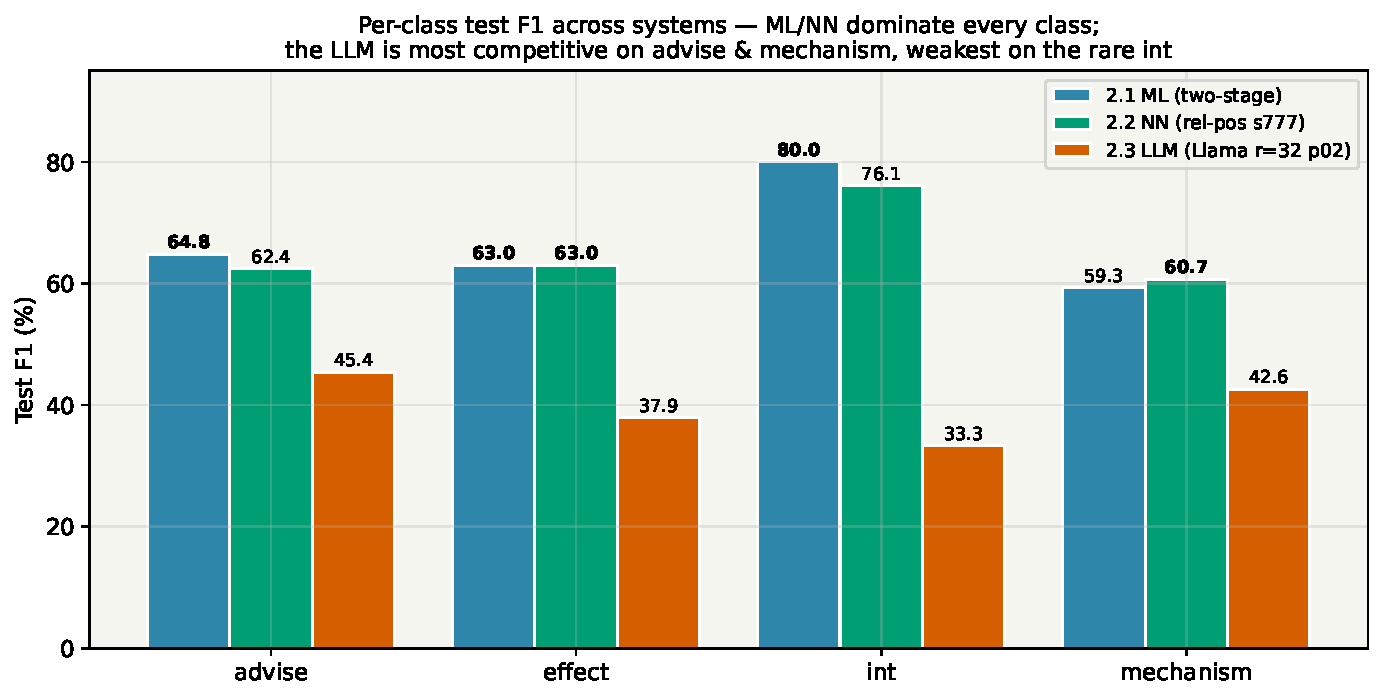
\includegraphics[width=\linewidth]{fig2_cross_perclass.pdf}
\caption{Per-class test F1 across systems.}
\end{subfigure}\hfill
\begin{subfigure}[t]{0.36\textwidth}
\centering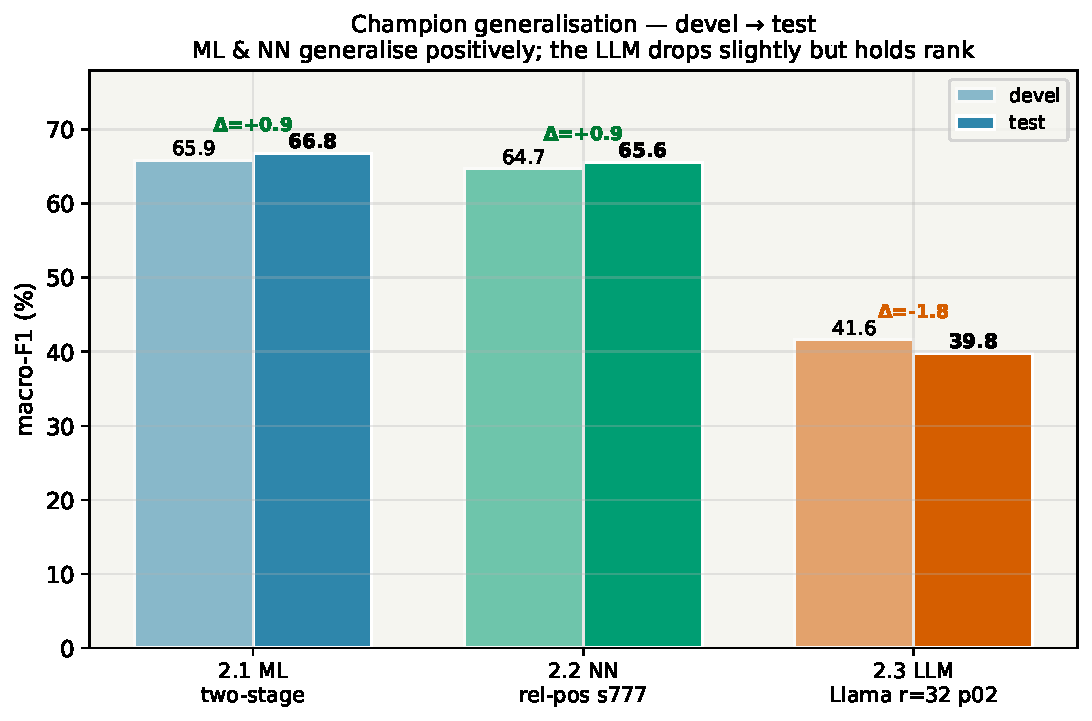
\includegraphics[width=\linewidth]{fig2_cross_devtest.pdf}
\caption{Champion devel$\to$test generalisation.}
\end{subfigure}
\caption{ML and NN dominate every class; the LLM is most competitive on \texttt{advise} and \texttt{mechanism} and weakest on the rare \texttt{int}. All three champions generalise sensibly from devel to test.}
\label{fig:cross2}
\end{figure}

\subsection{Trade-offs: effort, cost, explainability, controllability, performance}
The brief asks explicitly for a comparison across these five dimensions.

\begin{itemize}
\item \textbf{Development effort.} 2.1 required the most \emph{thinking}
(feature engineering: five mods, a solver/penalty sweep, the two-stage
decomposition) but each idea is a few lines and a 3-minute re-run. 2.2
was moderate (wiring four input channels, the relative-position
embedding, architecture flags). 2.3 was the \emph{least code} (env-var
knobs for LoRA rank and epochs, a second prompt file) but the longest
\emph{wall-clock} per idea by far.
\item \textbf{Computational cost.} 2.1 runs entirely on CPU: feature
extraction $\approx$3\,min, training in seconds --- the whole campaign is
minutes. 2.2 trains in $\approx$5--15\,min per seed on one GPU
($\approx$1\,h for a 5-seed audit). 2.3 is \textbf{two orders of
magnitude} more expensive: a single fine-tune is 1.5--5.4\,GPU-hours
and inference alone runs up to $\approx$5\,GPU-hours for Qwen; the full
LLM campaign consumed tens of GPU-hours and repeatedly hit the cluster's
disk quota.
\item \textbf{Explainability.} 2.1 is the most interpretable: the
learned feature weights are directly inspectable (\texttt{same-drug} is
the model's strongest signal; class-appropriate trigger verbs follow),
and every mod's effect has a concrete cause. 2.2 is intermediate
(input-channel ablations are interpretable; hidden states are not). 2.3
is the least: we can \emph{observe} that Qwen over-predicts under
\texttt{prompts02} but cannot point to why inside a 3B network.
\item \textbf{Controllability.} 2.3 offers the most direct behavioural
handles at inference (a one-line prompt swap visibly reshapes per-class
recall) --- but those handles are \textbf{brittle and non-transferable},
as the opposite Llama/Qwen prompt response shows. 2.1 is controllable
through its feature set and stage-1 threshold (a smooth, predictable
precision/recall dial); 2.2 only through architecture flags fixed at
training time.
\item \textbf{Performance.} On this task the ordering is unambiguous:
\textbf{2.1 ML (66.8) $\approx$ 2.2 NN (65.6) $\gg$ 2.3 LLM (39.8)} on
macro-F1. The classical pipeline wins.
\end{itemize}

\subsection{Why the LLM loses on DDI but won on NERC}
\begin{warnbox}\small
The same 3B LoRA recipe \emph{won} macro-F1 on Task~1 (NERC) yet trails
by $\approx$27\,pp here. Three structural reasons explain the reversal:
\textbf{(1) the task is relational}, not a surface property of one span
--- the answer depends on the syntactic relationship between two marked
drugs, which 2.1 encodes explicitly via dependency-path features and the
LLM must reconstruct from raw text; \textbf{(2) the 85\,\% \texttt{null}
imbalance} drives the LLM into systematic over-prediction (it labels
$\approx$29--64\,\% of true \texttt{null} pairs as positive), the single
largest error source; \textbf{(3) the output is a single token}, so the
LLM gets none of the structured-generation advantage that helped it on
the span-tagging NERC task. None of these is fixable by prompting at the
3B/4-bit scale our hardware allows.
\end{warnbox}

\subsection{When is each system the right choice?}
\begin{itemize}
\item \textbf{Use 2.1 (ML)} as the default for DDI: best macro-F1,
CPU-only, fully interpretable, minutes per iteration. On a relational,
syntax-driven task with hand-crafted dependency features, classical ML
is hard to beat.
\item \textbf{Use 2.2 (NN)} when a GPU is available and one prefers
learned representations to feature engineering; it reaches within 1.2\,pp
of ML without any hand-crafted syntactic features, and the
relative-position embedding is the key to getting there.
\item \textbf{Use 2.3 (LLM)} only where its flexibility (zero feature
engineering, natural-language control) outweighs a large accuracy and
cost penalty. At 3B/4-bit it is not competitive for DDI; a larger,
full-precision model might narrow the gap but would not change the
ranking on this hardware.
\end{itemize}

\paragraph{Overall conclusion.}
For DDI-2013 the three paradigms finish \textbf{2.1 ML = 66.8\,\%},
\textbf{2.2 NN = 65.6\,\%}, \textbf{2.3 LLM = 39.8\,\%} macro-F1. The
central, task-independent lesson --- consistent with Task~1 --- is that
\textbf{representation matters more than architecture}: in 2.1 a
feature \emph{combination} plus the two-stage decomposition delivered the
gains, in 2.2 the input channels and the relative-position embedding did,
and in 2.3 the LoRA rank and the prompt did. But the headline lesson is
the \emph{contrast} with NERC: a small fine-tuned LLM can match dedicated
systems on a span-extraction task, yet on a \emph{relational} task with
heavy class imbalance and syntactic signal, the classical
feature-based pipeline remains clearly ahead.

\end{document}
